\subsection{Introduction to Network Intrusion Detection System}
Network intrusion detection systems (NIDS) are the digital security guards of a network. NIDS observe the network communications (packets or flows) to detect and flag malicious activity or network policy violations in real time. In modern networks this role is complicated due to several factors such as (i) high data transfer rate of network connections of 100 Gbps and beyond; (ii) all data transferred over the network is encrypted with the latest encryption protocols such as TLS 1.3 (Transport Layer Security) and QUIC (Quick UDP Internet Connections); (iii) the rise of cloud-native, containerized workloads and elastic east-west traffic; and (iv) the increasingly data-driven decisions to be made by Security Operations Centres (SOCs) that require actionable and explainable alerts with low false positive rates \parencite{Zhou2024TLS13Survey,Cerasuolo2025Adaptable,KBS2025Datasets}.
 Meanwhile, open-source engines such as Suricata and Snort continue to dominate operational deployments, with commercial engines often embedding or extending these cores \parencite{SuricataDocs2025,SnortManual2024,CiscoSnort3Guide2024}.\\
 
\noindent NIDS can be categorized into two depending on how they monitor networks. There is signature-based detection which is a very rigid system and looks for specific, known malicious activities (like a security guard with a "most wanted" list). The anomaly-based detection are more flexible systems and look for anything that just seems "off". The smartest system today is hybrid approaches which combine both methods. Hybrid systems often use simple fast check to filter out the obvious threats and then pass the tricky stuff to more sophisticated, learning-based system for deeper analysis \parencite{Maseno2022HybridReview,Han2023HPNIDS,Naghib2025HybridReview}. These different approaches and their application in the real world are discussed in the following sections.

\subsection{How NIDS detect threats}
\subsubsection{Signature-Based Detection}
This is the most traditional way NIDS work. They are built on a library of rules that describe known attack patterns. For example, a rule might be, "If you see this exact sequence of bytes in a packet, it is a known virus". This approach offers high precision against known threats and provides interpretable and actionable alerts (for example CVE-aligned signatures with context) \parencite{SnortManual2024,SuricataDocs2025}. Its principal limitations are that this approach is useless against anything new or zero-day threats and keeping the rulebook up-to-date with the latest threats is never-ending task for security teams \parencite{Diana2025Overview,Han2023HPNIDS}. Modern signature-based engines overcome the performance concerns using multi-pattern matching (Ahp-Corasick variants), fast-path pre-filters and protocol parsers that normalize the inputs before rule evaluation \parencite{CiscoSnort3Guide2024}. Emerging work explores augmenting signature pipelines with machine learning to generalize patterns or prioritize rule subsets \parencite{Ahmed2025SignatureML}.\\

\noindent Snort is NIDS that operates primarily on a signature-based detection method. This approach, also known as misuse detection is based on matching network traffic against a predefined knowledge base of known attack vectors \parencite{Sadeghi2020ModernIDS}. The core of Snort's functionality is in its powerful detection engine which processes network packets continuously.\\

\noindent The Snort engine pipeline begins with a packet decoder that captures and normalizes raw packets from the network interface. This is followed by preprocessors that prepare the data for analysis, performing crucial tasks such as reassembling fragmented packets and TCP streams. The clean data is then passed to the detection engine, where it is evaluated against a comprehensive set of rules \parencite{CiscoSnort3Guide2024}. A Snort rule is a concise statement that defines a specific threat. It consists of a rule header, which specifies high-level criteria like the protocol and IP addresses, and rule options that provide granular, payload-level inspection. For an alert to be triggered, a packet must satisfy all conditions within both the header and the options, such as matching a specific byte pattern using the "content" keyword \parencite{SnortManual2024}. This logical AND operation ensures accurate and reliable detection. When a match occurs, Snort can log the event, alert an analyst, or, in an inline configuration and actively drop the malicious traffic.


\subsubsection{Anomaly-Based Detection}
Anomaly-based NIDS construct a model of normal traffic and flag anything that deviate from that normal traffic as malicious activity. In other words, instead of looking for what is bad, this approach learns what is normal on a network. It is like a security guard that knows everyone's daily routine and raises an alarm if someone shows up at 3 AM who has never been there before at that time. Techniques to detect the deviations from normal traffic ranges from statistical profiling and classical ML to deep neural architectures operating on sequences, graphs or learned embeddings of network events \parencite{ACM2024DLIDSReview,Diana2025Overview}. The main strength of this method is the ability to detect zero-day attacks. However the key weakness is that it generates lot of false positives espically when the network's normal behaviour changes (Concept drift) and it requires lot of high quality training data \parencite{KBS2025Datasets,AppliedIntelligence2025Benchmark}. Recent research targets adaptability (incremental/continual learning), transparency (XAI), and robustness to label scarcity and imbalance \parencite{Cerasuolo2025Adaptable,AppliedIntelligence2025Benchmark}.\\

\noindent While best known for its high-performance signature-based engine, Suricata's advanced features allows it to function it as an anomaly-based detection tool. Suricata's capabilities in approach are not limited to a single, built-in anomaly detection engine. It is instead relies on its ability to generate rich network telemetry that can be fed into external, learning-based systems. The output from this engine is in the form of EVE JSON, which includes flow metadata, file information and protocol specific details \parencite{SuricataDocs2025}.
This telemetry serves as the high-quality training and operational data for anomaly models. For example a machine learning model can be trained on this data to learn normal flow rates, packet sizes or protocol interactions. Deviation of live traffics such as sudden increase in a specific type of encrypted flow could be flagged as anomalous. This approach allows Suricata to act as data collection and preprocessing layer for a seperate more complex anomaly-based detection of zero-day attacks that would usually bypass signature-based detection tools \parencite{Han2023HPNIDS}.

\subsubsection{Hybrid Detection}
Hybrid NIDS all about getting the best of both methods. They use a combination of signature-based and anomaly-based methods to balance precision and speed \parencite{Maseno2022HybridReview,Naghib2025HybridReview}. A common setup include: (i) \emph{pipeline hybrids} where a fast signature check acts a first line of defense and only letting the suspicious traffics through a more complex anomaly detector; (ii) \emph{ensemble hybrids} which runs multiple detectors simultaneously (like a signature based engine, a flow analyser and an AI model) and then uses a smart system to combine the findings of individual detectors to make a final decision; (iii) \emph{multi-view hybrids}  where a joint of packets, flow, and contextual telemetry are used to overcome the limitation of single one \parencite{Qiu2022DSTHybrid}. For instance, a single suspicious packet (from a packet view) might be of a less concern but if it is part of a large unusual data transfer (from flow view) to server located in a known malicious location (from a contextual view). the system can more confident in its alert.
\emph{architectural} hybrids (section \ref{sec:deployment}) that combines  different detection systems or vantage points. Instead of using a single type of NIDS, this approach combines network-based detection with host-based and other telemetry to get a richer, more accurate picture of a potential threat and it provides a more comprehensive view of an organization's network security. 

\subsection{How NIDS are deployed in the real-world}\label{sec:deployment}
Deployment of NIDS in the real-world environments is a critical exercise in systems engineering.\\
\noindent Deployment strategies widely include:
\begin{enumerate}[label=\alph*)]
\item  Passive (out-of-band) using network Test Access Points (TAPs) or switch port analyzers (SPAN) / mirror ports to feed sensors. This avoids introducing inline latency or failure modes and suits detection-first postures \parencite{SuricataDocs2025}.
\item  Inline (IPS-capable) where sensors sit on the data path (e.g., NFQUEUE, AF\_PACKET, or hardware offload) and can drop or modify traffic \parencite{SuricataIPS2024,CiscoSnort3Guide2024}. Inline mode demands strict performance bounds and fail-open/fail-closed design.
\item  Cloud-native via Virtual Private Cloud (VPC) traffic mirroring and virtual taps (e.g., AWS VPC traffic mirroring, Azure VTAP); sensors run as VNFs or DaemonSets in Kubernetes. Elastic scaling and policy-as-code are key \parencite{Diana2025Overview}.
\end{enumerate}
diverse traffic acquisition methods, such as passive (out-of-band) monitoring via network TAPs or SPAN ports, which prevents inline latency \parencite{SuricataDocs2025}. Alternatively, NIDS can be deployed inline as Intrusion Prevention Systems (IPS), capable of discarding malicious traffic but at the same time demanding very strict requirements of speed, reliability and efficiency and fail-safe designs \parencite{CiscoSnort3Guide2024}. Operational success of NIDS further depends on integration with Security Information and Event Management (SIEM) and Security Orchestration, Automation, and Response (SOAR) platforms. 
This  makes it easier to connect different security alerts and add extra information to them and automated incident response workflows \parencite{Diana2025Overview}. Effective deployment thus extends beyond the detection engine to encompass a holistic security pipeline.

\subsubsection{Software and Hardware to boost performance}
To keep up with the modern super-fast networks, NIDS need to be able to detect every single packet in the network traffic. This requires a shift in programmable planes, which is essentially software or specialised hardware that can process network traffics at very high speed. On a regular server, technologies like extended Berkeley Packet Filter (eBPF)/ eXpress Data Path (XDP) acts like an efficient filter inside the operating system's kernel. They can catch network packets and send them directly to a NIDS for a quick scanning without having to make redundant copies. This saves lot of time and optimises the process efficiency \parencite{NSDI2023Electrode,ASPLOS2023eHDL}.\\
\noindent For higher speed networks, like on a specialised network cards or switches, a programming language called P4 is used. P4 let network engineers to create custom rules that can filter and analyse packets right on the hardware itself, before the packets even reach the main computer. This pre-analysis can quickly identify important traffic to send to more advanced detectors \parencite{P4NIDS2024}. These techniques shift computation closer to the packet path, reducing CPU cost and enabling higher-throughput deployments.

\subsubsection{Rule and Model Management} 
Signature-based systems needs to continuously update rules (e.g., community and commercial feeds) and careful policy selection (balanced vs.\ connectivity-biased) to manage alert volume \parencite{CiscoSnort3Guide2024,SuricataDocs2025}. ML-based NIDS introduce the additional challenges of dataset curation, label annotation, model retraining, and system rollbacks. MLOps practices such as data versioning, canary deployment, and drift monitoring are becoming standard in Security Operation Center (SOC) pipelines \parencite{ACM2024DLIDSReview,Cerasuolo2025Adaptable}.

Running a NIDS is an continuous effort. For signature-based systems, that means updating rules from threat intelligence feeds. For ML-based systems, that also involves the added maintenance of curating data, re-training models, and monitoring for drift that could make the model less effective.

\subsubsection{Integration with SIEM/SOAR} 
Operational success also depends on feeding normalized, enriched alerts (such as EVE JSON from Suricata) into Security Information and Event Management (SIEM) / Security Orchestration, Automation, and Response (SOAR) platforms for alert correlation, triage, and automated playbooks. Enrichment often includes asset context, identity, threat intelligence hits, and Packet Capture (PCAP) retrieval for forensic investigation \parencite{SuricataDocs2025,Diana2025Overview}.

\subsection{Datasets and Evaluation} 
Benchmarking of NIDS has long suffered from the lack of up-to-date or realistic corpora. A recent survey catalogs impressive progress, but highlights remaining gaps in corpus realism, label quality, and modern protocol coverage \parencite{KBS2025Datasets,AppliedIntelligence2025Benchmark}. For encrypted traffic in particular, community datasets like VisQUIC (QUIC/HTTP 3 traces with associated keying material for research) and ISP-scale QUIC backbone traces enable method development and also highlights privacy and reproducibility issues \parencite{VisQUIC2024,QUICBackbone2023}. Standardized preprocessing and publicly shared data are recommended to facilitate algorithmic comparisons \parencite{AppliedIntelligence2025Benchmark}.

\subsection{Contemporary Challenges} 
\subsubsection{Encryption and Protocol Evolution} 
TLS 1.3 encrypts more handshake fields and adds Encrypted ClientHello (ECH), reducing visibility into Server Name Indication (SNI) and other features long used for network analytics. QUIC moves transport semantics to user space over UDP and encrypts transport headers, complicating network function (middlebox) inspection and traffic classification \parencite{Zhou2024TLS13Survey,Enigma2025ETC}. For NIDS, these developments impact the visibility of deep packet inspection and shift focus toward side-channel features (timing, sizes, directions), JA3-like fingerprints for legacy contexts, and flow-based behavior over packet content \parencite{Zhou2024TLS13Survey,VisQUIC2024}. Researchers have proposed metadata signatures, semi-supervised learning, and auxiliary control-plane telemetry to recover discriminative power without payload decryption \parencite{EncryptedNIDS2022,VisQUIC2024,QUICBackbone2023}.

\subsubsection{Performance at Line Rate} 
Running NIDS at 40/100 Gbps+ line rates demands hard performance constraints on packet I/O, pattern matching, and model inference latency. Approaches include kernel-bypass I/O, hardware-friendly sketches, FPGA/SmartNIC offload, and continuously refined detection where cheap filters preserve headroom for expensive analysis \parencite{Han2023HPNIDS,NSDI2023Electrode,ASPLOS2023eHDL,P4NIDS2024}. Selecting tap points, sampling strategies, and feature extraction pipelines also matters to avoid excessive packet drops and maintain forensic utility.

\subsubsection{Data and Concept Drift} 
Enterprise traffic is non-stationary: software updates, new SaaS usage, and shifting organizational baselines all alter behavior. Adapting anomaly detectors over time requires avoiding uncontrolled false positives. Incremental and continual learning methods, explainable components, and human-in-the-loop feedback are under active research \parencite{Cerasuolo2025Adaptable,ACM2024DLIDSReview}. Robust drift-aware evaluation should include temporal splits and temporal adaptation protocols rather than random cross-validation \parencite{KBS2025Datasets}.

\subsubsection{Adversarial Robustness} 
Attackers may alter traffic to evade signatures (polymorphism, fragmentation) or ML models (adversarial examples, poisoning). Defenses include normalization and reassembly, robust feature sets, adversarial training, and cross-checking detectors in hybrid ensembles \parencite{Maseno2022HybridReview,Naghib2025HybridReview}. Programmable data planes can also help by enforcing sanitization at the edge to remove ambiguity before detection \parencite{P4NIDS2024}.

\subsubsection{Explainability and Analyst Trust} 
SOC analysts requires understanding why an alert fired to best prioritize response. Signature-based alerts are naturally explainable; ML-based alerts often are not. Integrating eXplainable AI (XAI) with incremental learning has been shown to improve transparency and maintain performance \parencite{Cerasuolo2025Adaptable}. In practice, coupling model outputs with example flows, contributing features, and historical context is also shown to speed up the classification.

\subsubsection{Operational Diffculties} 
Operating NIDS at scale involves manual alert review, tuning noisy rules, checking for rule regressions, and patching integration failures. Mature solutions in this space institutionalize change control for rules and models and automate continuous QA (e.g., staging sensors, mirrored traffic canaries) prior to production rollouts \parencite{CiscoSnort3Guide2024,SuricataDocs2025}. Inline deployments additionally require high-availability design  and SLA-aware fail-open policies for critical services \parencite{SuricataIPS2024}.

\subsection{Future Directions} 
First, encrypted-traffic analytics will continue to push for privacy-preserving features, federated learning and standardized benchmarks that respect legal constraints \parencite{Zhou2024TLS13Survey,VisQUIC2024}. Second, technologies like eBPF/XDP and P4 will allow network devices to be more self-sufficient. They'll be able to collect data and detect threats directly, which will speed up the entire process. \parencite{NSDI2023Electrode,P4NIDS2024,ASPLOS2023eHDL}. Third, hybrid systems will utilize XAI and active learning to better communicate between analysts and models, lowering false positives and improving time to detect \parencite{Cerasuolo2025Adaptable,Maseno2022HybridReview}. Finally, Building high-quality and constantly updated datasets (including QUIC/TLS 1.3 traffic) is critical for making impactful progress in network security research.
 \parencite{AppliedIntelligence2025Benchmark,KBS2025Datasets}.



% ML IN NIDS
\subsection{ML in Network Intrusion Detection Systems}

\subsubsection{Introduction} 
The ability to detect new and unknown attacks, as well as the scalability to handle large, high-speed data flows with high accuracy in today's threat environment have been identified as the most desirable capabilities for NIDS \parencite {agrawal2021survey}. To address these limitations, there has been significant research into the development of next-generation, more intelligent NIDS \parencite {aldhubaib2024network}. One of the most prevalent approaches that has emerged in this area is the use of machine learning techniques. ML techniques have the ability to learn and adapt to the traffic patterns they encounter without being explicitly programmed for each new threat. By doing so, ML can be used to create models that can detect both known and unknown attacks. This makes ML-based NIDS a promising solution, as it can be used to detect noval attacks. In this literature review, a comprehensive review of different machine learning techniques and algorithms and their applications in NIDSs are presented. The principles, methodologies, strengths, and limitations of each approach, with a particular focus on recent advances and challenges in the field are also discussed.

\subsection{Machine Learning Approaches in NIDS} 
Machine learning is a broad field that includes several different approaches. In the context of NIDS, this literature review focuses on and cover the supervised learning, unsupervised learning techniques and to a lesser extent, semi-supervised learning. 


\subsubsection{Supervised learning} 
Supervised learning is probably the most popular approach in NIDS \parencite {aldhubaib2024network}. As the name implies, supervised learning algorithms are provided with training data that is labeled with ground truth information. In the case of NIDS, this training data is a collection of network flow records of benign and various types of attacks. The task of supervised learning is to learn a function that maps the input features (network flow statistics, packet headers, etc.) to an output (i.e., class label), such as ‘Benign', ‘DoS', or ‘PortScan'. Once the function has been learned, it can then be used to label previously unseen records, that is, NIDS can predict a label for a given input of network flow. The success of supervised learning algorithms depends on the existence and use of data that is already labeled with ground truth, that is, information on the type of class a given record (network flow) belongs to. This labeled data is used to train the NIDS and is therefore a prerequisite for the use of the supervised learning approach.

Convolutional Neural Networks (CNNs) can be used in NIDS to process raw network packet data, where packets or sequences of packet features are mapped into a 1D or 2D grid. Convolutional layers can then learn spatial correlations within this data. For example, CNNs have been used to extract features from raw network payloads or flow-based time-series data \parencite {liu2023intrusion}.

\subparagraph{Strengths and Limitations} 
Strengths: This model is excellent at automatically learning key patterns directly from raw data. It can recognize patterns regardless of their position and builds up an understanding of complex structures by first identifying simpler features.
Limitations: Require large amounts of labeled data and computational resources for training, sensitive to the scale and normalization of input data, and may be overkill for simple patterns that do not benefit from deep representations.

\paragraph{Recurrent Neural Networks (RNNs)} 
RNNs are a class of neural networks designed for sequential data, with the ability to retain information in 'memory' over time through internal state feedback loops. This makes them well-suited for time-series data or any application where the current output depends on previous computations. In NIDS, RNNs can model temporal dependencies in network traffic to detect anomalies or attacks that unfold over time \parencite {zou2021survey}.

\subparagraph{Application in NIDS} 
RNNs, including variants like Long Short-Term Memory (LSTM) networks and Gated Recurrent Units (GRUs), are used to model time-dependent patterns in network traffic. They can effectively process sequences of network events or traffic flows to detect anomalies that develop over time, which is crucial for identifying complex, multi-stage attacks \parencite {al2020survey}.

\subparagraph{Strengths and Limitations} 
Strengths: Capable of capturing temporal dependencies and sequences in data, have internal memory to store past information, and can handle variable-length input sequences.
Limitations: Susceptible to the vanishing and exploding gradient problem during training, computationally intensive, and can be difficult to train for long sequences without modifications like LSTM or GRU cells.

\paragraph{Autoencoders} 
Autoencoders are neural networks used for unsupervised learning tasks, primarily for dimensionality reduction and feature learning. An autoencoder learns to compress (encode) the input data into a lower-dimensional representation and then reconstruct (decode) the data back to its original form \parencite {zou2021survey}.

\subparagraph{Application in NIDS} 
Autoencoders can be used for anomaly detection in NIDS by learning a compressed representation of normal network traffic. Once trained, the autoencoder attempts to reconstruct new data. High reconstruction errors can indicate anomalies, as the network has likely not learned to compress and reconstruct patterns associated with attacks \parencite {zou2021survey}.

\subparagraph{Strengths and Limitations} 
Strengths: Effective for dimensionality reduction and feature learning, can be used for anomaly detection by learning to reconstruct normal traffic patterns, and relatively simple to implement and train.
Limitations: Require a well-defined notion of "normal" data for training, can be sensitive to the selection of the bottleneck layer's size, and may not perform well if the data is too noisy or the network is too complex.

\paragraph{Variational Autoencoders (VAEs)} 
Variational Autoencoders are a type of generative model that not only learns to encode and decode data like traditional autoencoders but also imposes a probabilistic structure on the latent space. VAEs are trained to maximize the likelihood of the data while regularizing the latent space to approximate a prior distribution, often a Gaussian \parencite {al2020survey}.

\subparagraph{Application in NIDS} 
VAEs can be applied in NIDS for anomaly detection by learning the distribution of normal network traffic. They are particularly useful when the model needs to generate new data points that are similar to the input data, such as simulating network traffic or generating adversarial examples for testing \parencite {al2020survey}.

\subparagraph{Strengths and Limitations} 
Strengths: Can generate new data points similar to the training data, provide a probabilistic approach to encoding data, and can be used for anomaly detection and data imputation.
Limitations: Training can be more complex due to the need to balance reconstruction loss with the regularization of the latent space, may struggle with representing complex data distributions without enough latent variables, and require careful tuning of the network architecture and hyperparameters.

\subparagraph{Strengths and Limitations} 
Strengths: Automatic feature extraction, invariance to input variations, effective for large and complex datasets. Ability to capture spatial dependencies in data representations.
Limitations: Require large labeled datasets for training, computationally intensive (particularly for very deep networks), less interpretable than some other models. Need data transformation for network data to fit the grid-like input requirement.

\paragraph{Recurrent Neural Networks (RNNs) and their Variants (LSTM, GRU)}
RNNs are designed to handle sequential data, which makes them well-suited for time series analysis, like network traffic that exhibits temporal dependencies. Standard RNNs, however, struggle with long sequences due to vanishing/exploding gradient problems. LSTM and GRU are RNN variants that use gating mechanisms to control information flow, allowing them to capture long-term dependencies in sequential data \parencite {zhao2022anomaly}.

\subparagraph{Application in NIDS} 
LSTM and GRU can be used in NIDS that represent network traffic as a sequence of events (e.g., packets in order within a flow, or a sequence of flows) because they can learn the temporal behaviour of entities in the network and spot anomalies as deviations from the learned temporal patterns. This is particularly useful for detecting multi-stage attacks or attacks that follow certain event sequences \parencite {yin2023intrusion}.

\subparagraph{Strengths and Limitations} 
Strengths: Great for sequential data and long-term temporal dependencies. Suitable for time-dependent attack detection. 
Limitations: Computationally heavy and slow to train for long sequences. Still can be hard to interpret, and require careful architecture and hyperparameter tuning.

\paragraph{Autoencoders (AEs)} 
Autoencoders are unsupervised neural networks used for dimensionality reduction and learning efficient codings of data in an unsupervised way. They consist of an encoder, which maps the input data to a lower-dimensional latent space representation, and a decoder, which reconstructs the input data from this latent space. If trained on benign data, an AE should be able to reconstruct normal patterns well, while anomalies (unseen or rare data) will have high reconstruction errors \parencite {bendre2023comprehensive}.

\subparagraph{Application in NIDS} 
Autoencoders are used in NIDS for anomaly detection. By training an AE on benign network traffic, it learns the patterns of normal traffic. When a new network flow is passed through the AE, a high reconstruction error would indicate that the flow is an anomaly \parencite {bendre2023comprehensive}. This can be a form of unsupervised anomaly detection, suitable for zero-day threats.

\subparagraph{Strengths and Limitations}
\noindent Strengths: Can be used for unsupervised anomaly detection, can learn complex non-linear relationships, and is useful for dimensionality reduction. Can be robust if trained on diverse benign traffic.
Limitations: Depends on architecture and hyperparameters. High reconstruction error doesn't always mean malicious anomaly, can lead to false positives on legitimate but novel traffic. Requires sufficient normal data for training \parencite{said2023systematic}.

\paragraph{Generative Adversarial Networks (GANs)}
\noindent GANs involve two neural networks, a generator (G) and a discriminator (D), competing in a minimax game \parencite{goodfellow2014generative}. The generator's job is to produce synthetic data that resemble the real data as closely as possible, while the discriminator's job is to differentiate between real and fake data. The adversarial training process drives both networks to improve iteratively \parencite{elsayed2021survey}.


\subparagraph{Application in NIDS} 
GANs can be used in NIDS for several purposes. One is data augmentation , generating synthetic attack samples to address the class imbalance in the training dataset, especially for rare attack types \parencite {kim2021adversarial}. Another application is for anomaly detection , where the discriminator, trained to distinguish real benign data from fake data, can flag malicious samples as “fake” or highly different from the normal data distribution \parencite {liu2023intrusion}.

\subparagraph{Strengths and Limitations} 
Strengths: Can produce highly realistic synthetic data for data augmentation, potentially improving the ability to detect rare attacks. The discriminator can serve as a powerful anomaly detector.
Limitations: Extremely difficult to train (mode collapse, training instability), sensitive to hyperparameters, and computationally expensive. Generating meaningful and diverse attack samples for NIDS use cases is still an active research area.

\subsubsection{Semi-Supervised Learning} 
Semi-supervised learning is a hybrid learning technique that uses a small amount of labeled data with a large amount of unlabeled data during training. It lies somewhere between supervised and unsupervised learning and can be particularly useful in scenarios where labeling data is expensive or time-consuming but unlabeled data is plentiful. Semi-supervised learning has been successfully applied to a variety of problems in NIDS, and it is an area of active research.

\subparagraph{Application in NIDS} 
In the context of NIDS, semi-supervised learning can use the small labeled dataset to provide an initial framework of what is normal and what is malicious. The model can then use this as a starting point to infer the labels of the unlabeled data, or to adjust its own structure in an unsupervised way, thereby enhancing its overall performance and generalization abilities \parencite {zou2021survey}. Common semi-supervised learning techniques include self-training (where the model labels its own most confident predictions) or co-training (where multiple models are trained on different views of the data).

\subparagraph{Strengths and Limitations} 
Strengths: Lessens the dependence on large labeled datasets, making it more practical for NIDS where labeling is expensive. Can lead to better model generalization by leveraging large amounts of unlabeled data.
Limitations: Can be sensitive to the quality of the initial labels. Errors in self-labeling can propagate and worsen model performance. The assumptions made about the data distribution (e.g. the cluster assumption) may not always hold true.

\subsection{Challenges and Future Directions of ML in NIDS}
Despite these remarkable achievements, the application of machine learning to NIDS is associated with a number of important and, in some cases, severe challenges \parencite{sharafaldin2018survey, al2020comprehensive}. The tasks of addressing the challenges and opening future research and application directions for ML-based NIDS form the core of the relevant work streams in the domain.

\subsubsection{Data Imbalance} 
Network intrusion datasets, including CIC-IDS2017, are notoriously highly imbalanced \parencite {sharafaldin2018toward}. Benign traffic makes up the vast majority of samples, while the instances of actual attacks, particularly rare and sophisticated ones (e.g., Heartbleed, Infiltration), constitute only a tiny fraction. This extreme imbalance can lead to ML models that are strongly biased toward the majority class (benign), resulting in high overall accuracy but very poor detection rates (low recall) for the important minority attack classes \parencite {agrawal2021survey}. A NIDS that misses most actual attacks is practically useless, no matter how high its overall accuracy is.

\subparagraph{Mitigation Strategies} 
A number of techniques can be used to mitigate data imbalance:
\begin{itemize}[noitemsep] 
\item Resampling Techniques: Include oversampling the minority class (e.g., SMOTE - Synthetic Minority Over-sampling Technique, ADASYN - Adaptive Synthetic Sampling) to create synthetic samples for the minority class, or undersampling the majority class (e.g., Random Undersampling, Tomek Links, Edited Nearest Neighbours) to remove samples from the majority class \parencite {mahfouz2022systematic}.
\item Cost-Sensitive Learning: Modifying the learning algorithm to assign higher misclassification costs to the minority class errors. For example, XGBoost can use the scale\textunderscore pos\textunderscore weight parameter \parencite {habeeb2024two}.
\item Ensemble Approaches: Designing ensemble models to specifically handle imbalance, like Balanced Bagging or EasyEnsemble.
\end{itemize} 
Ongoing research continues to explore more sophisticated and adaptive resampling techniques, particularly for multi-class imbalanced scenarios, and the development of imbalance-aware loss functions.


% CIC-IDS2017 

\subsection{Exploratory Data Analysis (EDA) of the CIC-IDS2017 Dataset} 

\subsubsection{Brief Introduction} 
It is an undisputable fact that the quality of a ML model, in this case, a NIDS, ultimately reflects the quality of the training data and its most pertinent attributes. A prior EDA of the dataset at hand is, thus, a necessary and essential preliminary step in the development and optimisation of a powerful NIDS model. By exploring the data, in general, and understanding its particular structure, contents, and statistical properties, in particular, a strong foundation is set for further, more targeted and advanced data pre-processing techniques, as well as for the informed selection of a suitable ML model. As the CIC-IDS2017 dataset is the primary data source of this NIDS experiment, a closer look at its most important properties is taken. A more thorough understanding of its advantages and limitations can help make even more critical decisions at subsequent stages of the ML model development.

In this sectiion shows how CIC-IDS2017 dataset is being explored and understood better. First background and key characteristics has been described. Then, a summariy the high-level observations collected while inspecting the data is presented. After that, the main challenges and issues that were faced and expect to still face in using the chosen dataset for the purpose of building an ML-based NIDS is presented. Finally, a general and practical information about CIC-IDS2017 is also included. The primary purpose of the present section is to extract important, actionable insights that will directly inform further work throughout the entire remainder of this dissertation.

\subsubsection{The CIC-IDS2017 Dataset: Background and Key Characteristics} 
The CIC-IDS2017 dataset is a relatively recent dataset among contemporary NIDS research and practice. It was developed by the Canadian Institute for Cybersecurity (CIC) at the University of New Brunswick (UNB) \parencite {sharafaldin2018toward}. The CIC-IDS2017 dataset was designed with the intent to remedy the key problems of previous, outdated, and often synthetic datasets, such as KDD Cup 99 or NSL-KDD. Namely, unlike its predecessors, it aimed to better represent the diversity, scale, and continuously evolving nature of modern network traffic and attack scenarios \parencite {agrawal2021survey}. The designers of CIC-IDS2017, thus, paid special attention to both generating realistic background traffic and executing a set of up-to-date attack scenarios. This set of considerations was incorporated into the data collection in an attempt to mirror the challenges that NIDS encounter in the real world \parencite {aldhubaib2024network}.

The dataset was collected over five days, from Monday, July 3, 2017, to Friday, July 7, 2017. During this period, both normal and malicious network activities were recorded. The network topology aimed to simulate a standard enterprise network and included the following: a firewall, various switches and routers, and a mixture of different operating systems (Windows, Ubuntu, and Mac OS X) on the victim and attacking network. The heterogeneity of the setup was meant to account for a larger variety of interactions, including within-LAN (internal) and outside (internet) traffic \parencite {kumar2021cicids}. The benign traffic, especially crucial for building a viable anomaly detector, was generated by simulating and tracking the abstract naturalistic behaviours of 25 individual users. These users were engaged in everyday online activities, such as web browsing (HTTP, HTTPS), file sharing (FTP), secure remote shell (SSH), and regular email use. The profiling was meant to result in naturalistic benign traffic, an essential ingredient for any supervised or unsupervised learning model attempting to differentiate between normal and abnormal behaviour.

The attacks were selected based on prevalent threat reports in 2016 and their expected relevance to the current cyber threat landscape. They were also staged throughout the collection period, from Tuesday to Friday, to monitor their effects on the live network. The included attacks are as follows: 
\begin{itemize}[noitemsep] 
\item Brute Force FTP \& SSH: These are persistent attempts to access the FTP and SSH services by trying a large number of username-password combinations.
\item DoS (Denial of Service): A category of attacks primarily aimed at taking an online service down. A list of the DoS attacks, especially prevalent ones, included in the dataset, such as GoldenEye, Hulk, Slowhttptest, and Slowloris.
\item DDoS (Distributed Denial of Service): A coordinated and usually more severe version of DoS attacks but launched from various geographically distributed or compromised machines.
\item Heartbleed: An attack that involved the exploitation of the critical vulnerability in the OpenSSL cryptographic library.
\item Web Attack: This category includes attacks targeting web applications and their common vulnerabilities. The web-based attacks, in particular, included in the dataset are brute force attack (password guessing), XSS (cross-site scripting), and SQL injection.
\item Infiltration: This category of attacks represents intrusion attempts to access or steal data from an organisation's internal network.
\item Botnet: A botnet is a network of internet-connected devices ( bots'') that have been compromised and controlled by a single malicious entity, called a bot-herder''.
\end{itemize} 
The diversity and comprehensiveness of the attacks used to construct the dataset, combined with the orchestrated realistic benign traffic, make CIC-IDS2017 especially suitable for modern NIDS research. This enables ML models to be developed, evaluated, and optimised in a setting that closely resembles real-world conditions \parencite {al2022cicids}.

\subsubsection{Structure and Features} 
The CIC-IDS2017 dataset comes in two main variants: raw PCAP (Packet Capture) files and processed CSV (Comma Separated Values) files. The PCAP files, however, are at a lower level of detail, so the processed CSV files, which contain the already pre-extracted network flow features, are the ones more commonly used for ML applications \parencite {sharafaldin2018toward}. The CSV files, in their turn, were processed by the dedicated CICFlowMeter tool, capable of extracting a rich set of more than 80 features for each of the observed network flows. For reference, the very network flow is defined as a sequence of related packets travelling from a particular source to a particular destination. A network flow is usually identified by a 5-tuple: a source IP address, a destination IP address, a source port number, a destination port number, and the protocol number.

Each row of the CSV files, therefore, contains a single, unique network flow. This network flow is characterised by an associated timestamp and a set of numerical and categorical features. From the original 84 available features, a small portion will likely be removed after an initial inspection and in light of the relevant literature. This is because some of the feature columns will have near-zero variance (i.e. the same values for almost all samples) and can thus be safely removed from further consideration \parencite {kumar2021cicids}. The main feature categories are the following: 
\begin{itemize}[noitemsep] 
\item Basic Features: The basic information about a flow, such as Protocol (TCP, UDP, ICMP), Flow Duration (how long the flow lasted), Total Fwd Packets (the number of packets in the forward direction), and Total Backward Packets (the number of packets in the backward direction).
\item Flow Features: These features describe the overall behaviour and rates of the flow. The most commonly used ones are Flow Bytes/s , Flow Packets/s , Flow Inter-Arrival Time (IAT) Mean , and Flow IAT Standard .
\item Statistical Features of Packet Lengths: These features describe the distribution of packet sizes in the flow and include Min Packet Length , Max Packet Length , Packet Length Mean , and Packet Length Std . These features are useful for identifying fragmented or unusually large/small payloads.
\item Time-Based Features (IAT): These capture the time intervals between packets and include features such as Fwd IAT Mean and Bwd IAT Std , which can be used to detect regular or periodic packet transmission.
\item Flag Counts: These represent the count of specific TCP flags within a flow, such as Fwd PSH Flags , Bwd PSH Flags , Fwd URG Flags , and Bwd URG Flags . These flags often indicate control operations like connection establishment, termination, or the transmission of urgent data.
\item Header Lengths: These include features such as Fwd Header Length and Bwd Header Length which record the sum of lengths of headers for the forward and backward packets, respectively.
\item Target Label: This is the final, non-feature column, called Label , that records the ground truth. It contains either the label 'BENIGN' if a particular row of the dataset represents normal network activity or a particular attack type (e.g. 'DoS Hulk', 'PortScan', 'DDoS', 'Web Attack-XSS', etc.) if not. 
\end{itemize} 
The pre-extracted, rich set of flow-based features, thus, allows the researcher to significantly speed up the first, preliminary stages of model development. It, instead, frees up some time and resources for more focused work on more advanced ML-related and, often more pressing, problems, such as the choice of the right algorithm and its further, more in-depth, hyperparameter optimisation, as well as for a more careful evaluation of the results \parencite {shafi2022comprehensive}. However, the actual quality, relevance, and possible interdependencies of the features and their impact on a chosen ML model can and should still be carefully investigated in a more thorough exploratory data analysis.

\subsubsection{Dataset Overview} 
We are now in a position to present an overview of the CIC-IDS2017 dataset in numbers, with some high-level descriptive statistics, as well as, with the main characteristics collected from our initial EDA.

Table \ref{tab: flow_counts} shows the total number of normal and anomalous network flows in each of the five collection days. We can see that Friday features the highest number of benign flows (around $2.5\times10^6$), and Monday is the least populated, with about $2\times10^6$. Moreover, there are a noticeably larger number of anomalous network flows on Thursday and Friday. This may be due to a higher number of background services and users performing their tasks throughout the week or simply a coincidence. It can also be noted that, overall, benign flows outclass anomalous ones, with the anomalous data accounting for less than 5\% of all CIC-IDS2017 network flows.

\begin{table}[h] 
\centering 
\caption{Normal and Anomalous Flow Counts per Day} 
\label{tab:flow_counts} 
\begin{tabular}{lcc} 
\toprule 
Day of Week & Normal Flows & Anomalous Flows \\ 
\midrule 
Monday & $1.95\times10^6$ & $3.05\times10^4$ \\ 
Tuesday & $2.17\times10^6$ & $4.56\times10^4$ \\ 
Wednesday & $2.18\times10^6$ & $3.89\times10^4$ \\ 
Thursday & $2.27\times10^6$ & $6.84\times10^4$ \\ 
Friday & $2.47\times10^6$ & $6.92\times10^4$ \\ 
\bottomrule 
\end{tabular} 
\end{table} 

Table \ref{tab: data_percentages} and Figure \ref{fig:data_count} show the respective numbers and relative proportions of benign and anomalous data. From these figures, we can quickly see that, indeed, we are working with a quite imbalanced dataset, with the malicious data far outnumbered by the benign traffic data. In other words, the number of anomaly samples is about five times smaller. This degree of imbalance is undesirable in the given context, so, at some point later, we will consider implementing various resampling methods to rebalance the dataset.

\begin{table}[h] 
\centering 
\caption{Count and Proportion of Normal and Anomalous Traffic Data}
\label{tab:data_percentages} 
\begin{tabular}{lcc} 
\toprule 
Flow Type & Count of Data Points & Percent of Total Data \\
\midrule 
Normal & $1.18\times10^7$ & 95.173\% \\ 
Anomalous & $6.11\times10^5$ & 4.827\% \\ 
\bottomrule 
\end{tabular} 
\end{table} 

\begin{figure}[H] 
\centering 
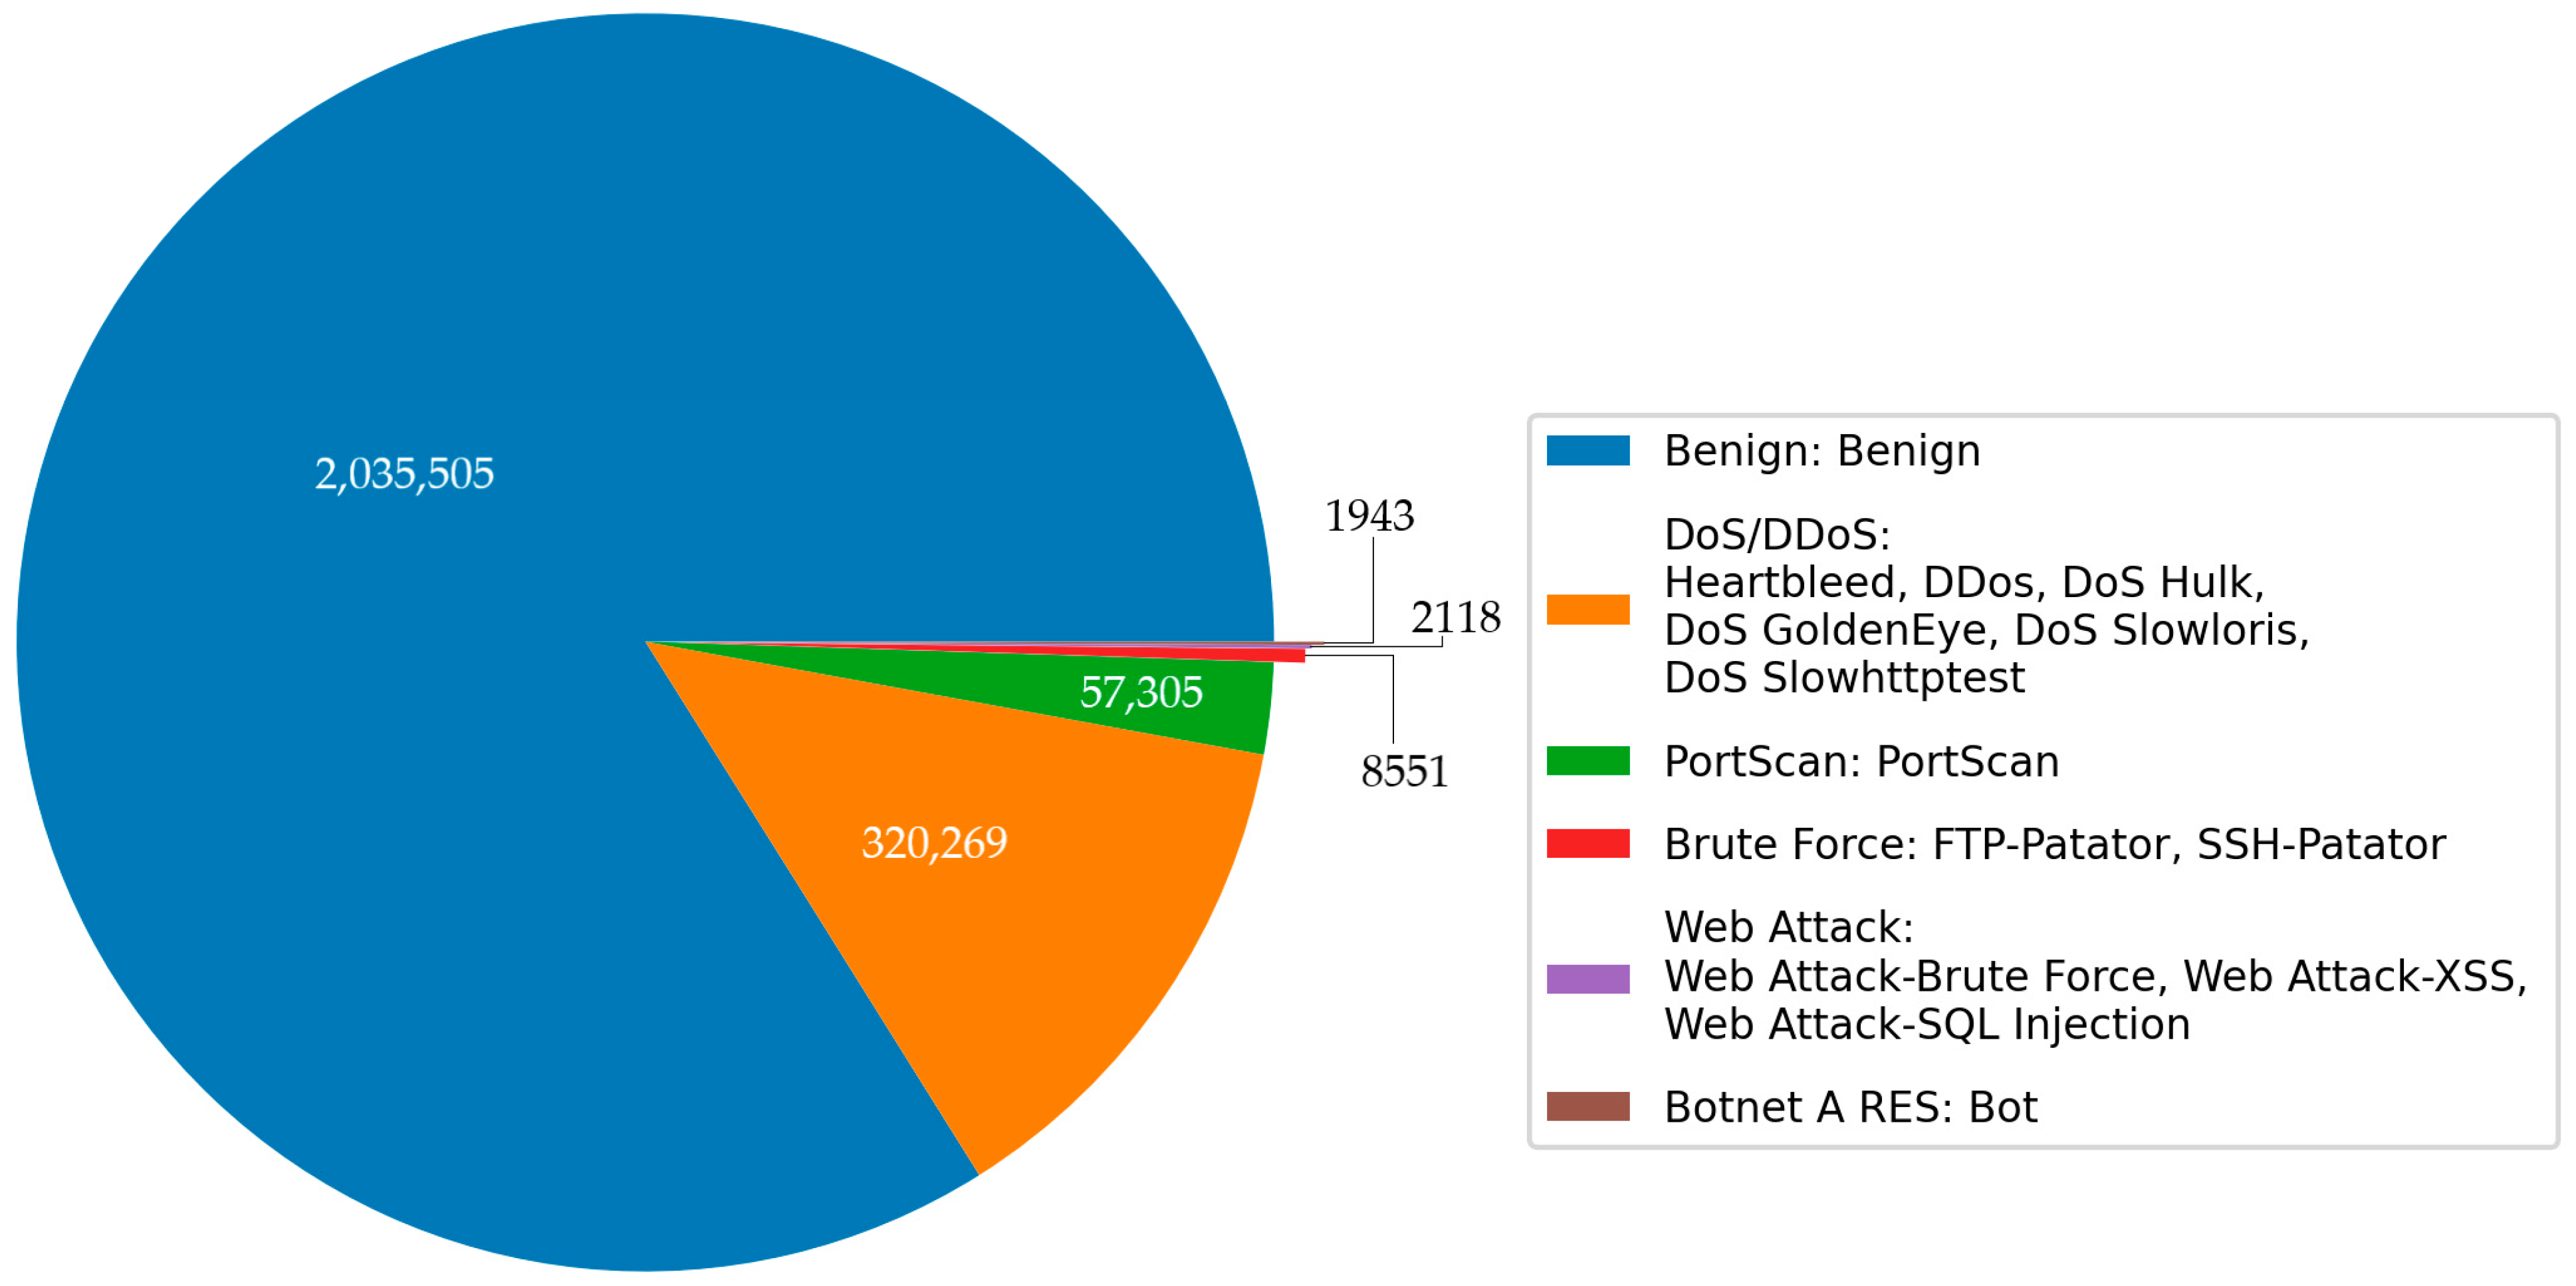
\includegraphics[width=0.75\textwidth]{assets/figures/data_count.png} 
\caption{Pie chart showing the count of normal and anomalous data}
\label{fig:data_count} 
\end{figure} 
\parencite{s23218788}

Figure \ref{fig: class_distr} and Table \ref{tab:class_distr} display a similar view of the CIC-IDS2017 dataset's class distribution, now for individual, specific anomaly types. It can be seen that DoS attacks, including DDoS attacks, are the most prevalent anomalous class, with over a thousand samples. In fact, among anomalous network flows, they constitute over 40\% of all data points. The least prevalent anomalies in the dataset are Heartbleed, Botnet, and Web Attack-XSS, each with only a few dozen samples. While Heartbleed has only one single instance in the dataset, both Botnet and Web Attack-XSS have over 20 observations each.

This observed, uneven distribution of data among the available anomaly types is the result of both real-world conditions and the focused choice of the dataset's creators. In other words, more dangerous and severe attacks tend to be more prevalent. In contrast, less frequent, more specialised and opportunistic, or weaker attacks are usually rarer and, hence, less well-represented in the resulting datasets. This is also why the chosen CIC-IDS2017 dataset was not completely rebalanced among all available classes, as the degree and direction of the available class rebalancing would likely misrepresent the real conditions.

\begin{figure}[H] 
\centering 
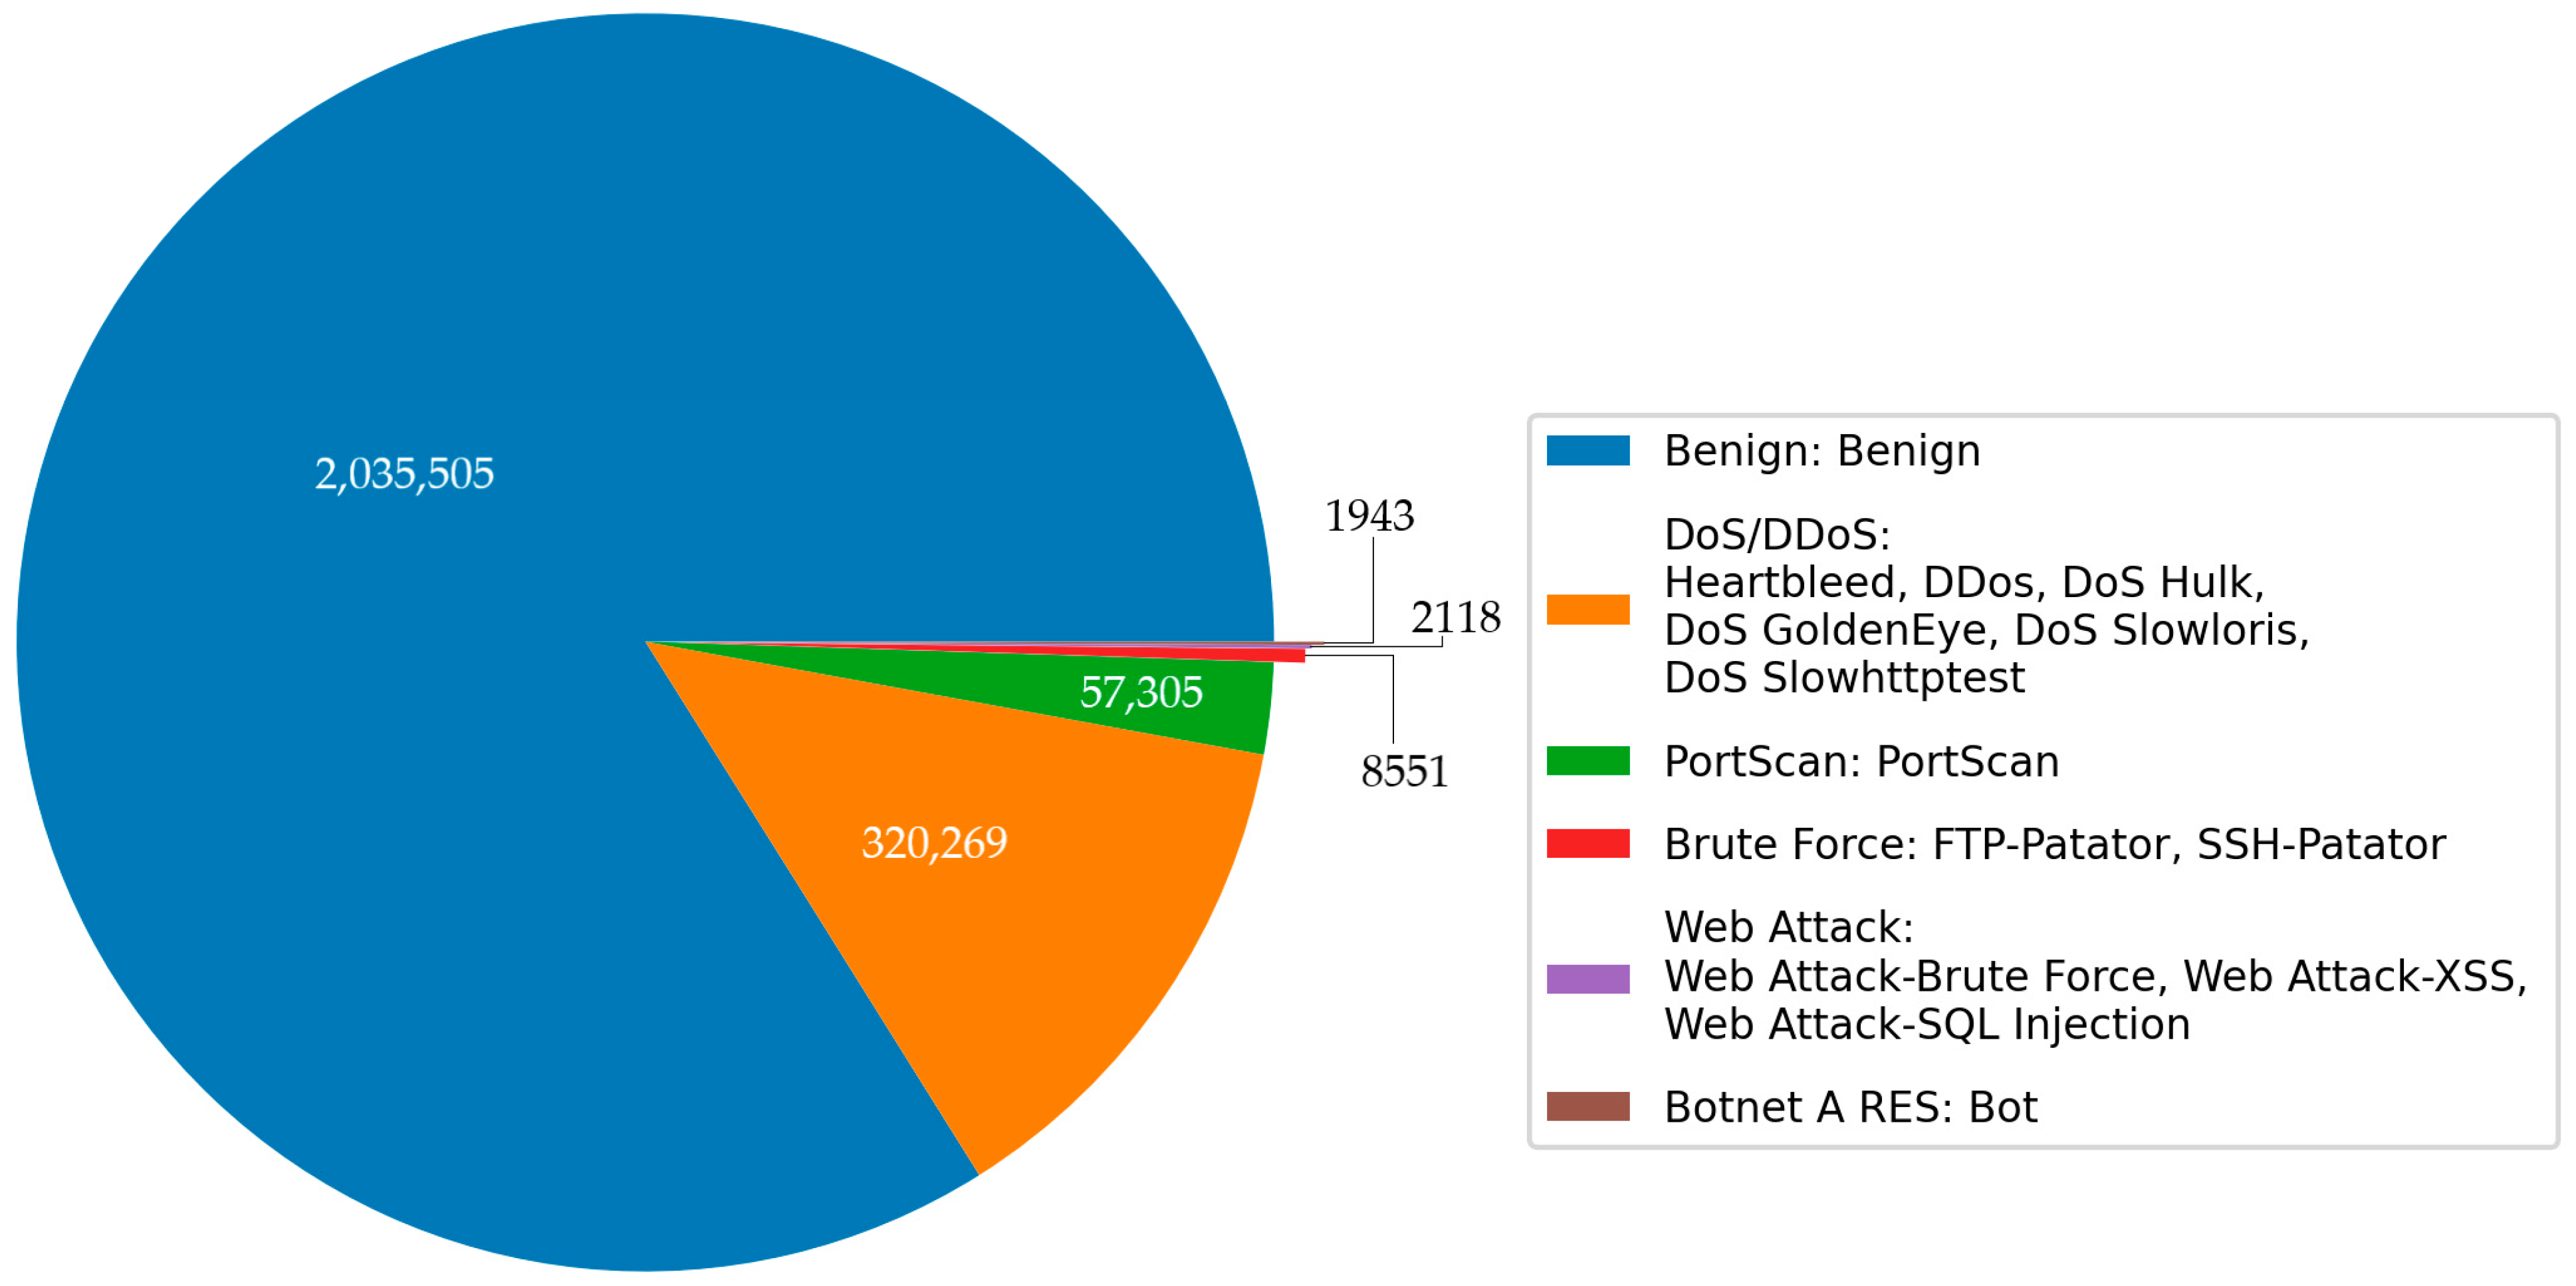
\includegraphics[width=0.75\textwidth]{assets/figures/class_distr.png} 
\caption{Pie chart showing the distribution of CIC-IDS2017 anomaly types}
\label{fig:class_distr} 
\end{figure} 
\parencite{s23218788}

\begin{table}[H] 
\centering 
\caption{Distribution of Anomaly Types in the CIC-IDS2017 Dataset}
\label{tab:class_distr} 
\begin{tabular}{lll} 
\toprule 
Type of Anomaly & Count & Percent of Anomalous Traffic \\
\midrule 
Botnet & 44 & 7.19\% \\ 
Brute Force FTP & 155 & 25.32\% \\ 
Brute Force SSH & 156 & 25.47\% \\ 
DoS & 764 & 124.83\% \\ 
DDoS & 576 & 94.02\% \\ 
Heartbleed & 1 & 0.16\% \\ 
Infiltration & 265 & 43.29\% \\ 
Web Attack-XSS & 48 & 7.84\% \\ 
\bottomrule 
\end{tabular} 
\end{table} 

Figure \ref{fig: dataset_shape} and Table \ref{tab:dataset_shape} show the detailed shape of the CIC-IDS2017 dataset in the form of the exact number of samples, features, and the expected number of missing values, if any.

As already discussed, the total number of CIC-IDS2017 samples is close to $1.25\times10^7$. The number of features is 79, as we expect to later remove at least the single isyn identification'' feature due to its near-zero variance. The number of missing values, in turn, is 0, which is to be expected, as this was supposed to be taken care of by the pre-processing step of CICFlowMeter.

\begin{figure}[H] 
\centering 
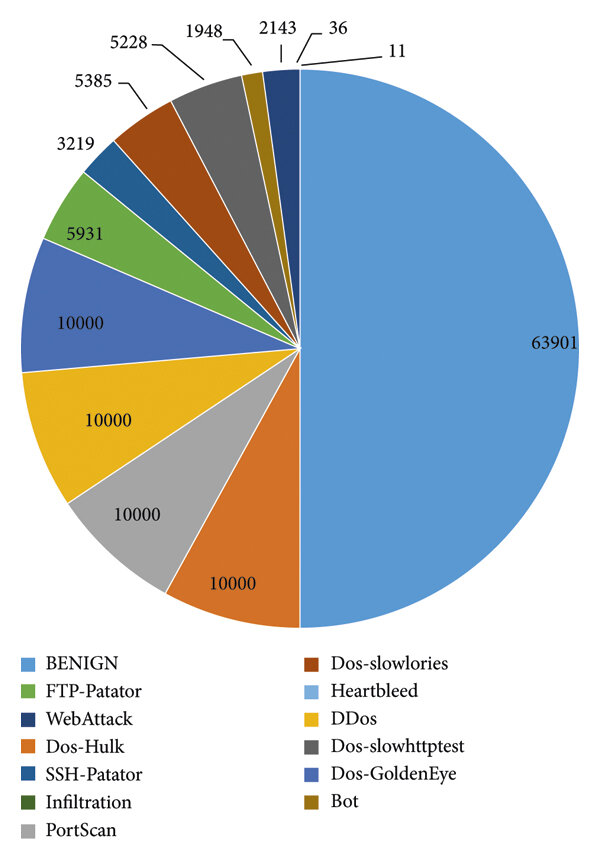
\includegraphics[width=0.5\textwidth]{assets/figures/dataset_shape.jpg} 
\caption{Shape of the CIC-IDS2017 dataset} 
\label{fig:dataset_shape} 
\end{figure} 
\parencite{articl5432e}

\begin{table}[H] 
\centering 
\caption{Dimensions of the CIC-IDS2017 Dataset} 
\label{tab:dataset_shape} 
\begin{tabular}{lrrr} 
\toprule 
{} & Samples & Features & Missing Values \\ 
CIC-IDS2017 Dataset & $1.25\times10^7$ & 79 & 0 \\ 
\bottomrule 
\end{tabular} 
\end{table} 

Table \ref{tab:dataset_classes} and Figure \ref{fig:dataset_distr} below summarise the categorical nature of the CIC-IDS2017 target label in more detail. It is, once again, confirmed that the available labels in CIC-IDS2017 include benign traffic as well as 11 unique anomalies or attack types.

\begin{table}[h] 
\centering 
\caption{Classes in the CIC-IDS2017 Dataset} 
\label{tab:dataset_classes} 
\begin{tabular}{lr} 
\toprule 
Type of Traffic & Count of Samples \\ 
\midrule 
Normal/Benign & $1.18\times10^7$ \\ 
DoS Attack & 764 \\ 
DDoS Attack & 576 \\ 
Brute Force FTP & 155 \\ 
Brute Force SSH & 156 \\ 
Heartbleed Attack & 1 \\ 
Infiltration Attack & 265 \\ 
Botnet Traffic & 44 \\ 
Web Attack (XSS) & 48 \\ 
DoS Hulk Attack & 157 \\ 
SlowHTTPTest Attack & 55 \\ 
Slowloris Attack & 132 \\ 
PortScan Attack & 292 \\ 
Web Attack (Brute Force) & 129 \\ 
GoldenEye DDoS Attack & 191 \\ 
\bottomrule 
\end{tabular} 
\end{table} 

\begin{figure}[H] 
\centering 
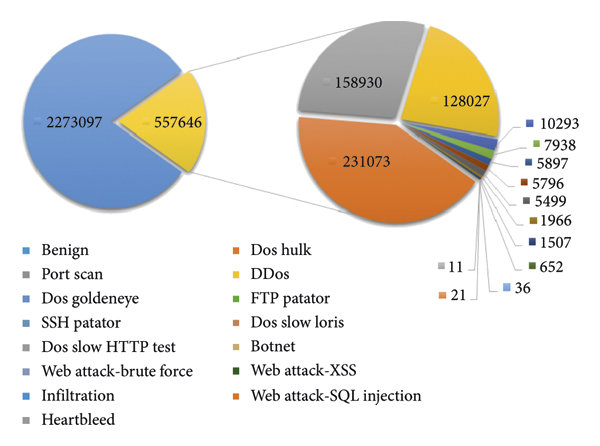
\includegraphics[width=0.75\textwidth]{assets/figures/dataset_distr.jpg} 
\caption{Distribution of CIC-IDS2017 classes} 
\label{fig:dataset_distr} 
\end{figure} 
\parencite{article5672}

Table \ref{tab: dataset_correlations} and Figure \ref{fig:dataset_heatmap} visualise the correlations between features in CIC-IDS2017 in the form of a heatmap. These correlations are also summarised in the table below for the top 15 features that display the highest correlation with the target class.

We can notice several important tendencies from this plot, the most notable of which is a strong correlation between many features. This is, however, a somewhat expected outcome, as the feature set was extracted from the raw data by the very same tool and is likely to have non-zero, although low to moderate in this case, interdependencies and associations. This will likely become even more of an issue in the chosen XGBoost model, as it, unlike some other ML models, will likely be affected by feature duplication and redundancy. It will be left to the feature importance'' analysis to reveal whether these multi-directional feature dependencies will ultimately become a threat to the robustness of the resulting ML models.

The important observation, however, is that there are no such significant correlations between features and the target class. In other words, no feature is expected to be clearly better or more informative than all the others, which is, in turn, an ideal state of affairs. In practical terms, it means that we will not expect a priori knowledge of the impact of any one feature on the result.

\begin{table}[H] 
\centering 
\caption{Correlations with the Target Class in the CIC-IDS2017 Dataset}
\label{tab:dataset_correlations} 
\begin{tabular}{lr} 
\toprule 
Feature & Correlation with Target Class \\ 
\midrule 
Fwd PSH Flags & 0.006668 \\ 
Bwd PSH Flags & 0.010292 \\ 
Back Hour & -0.025607 \\ 
Avg Fwd Segment Size & 0.008463 \\ 
Avg Bwd Segment Size & 0.004851 \\ 
Init Fwd Win Byts & 0.022085 \\ 
Fwd Header Len. Variation & -0.027403 \\ 
Max Fwd PSH Flags & 0.024079 \\ 
Flow Duration & 0.000168 \\ 
SourcePort & 0.037022 \\ 
Dst Host Droplet 173 & -0.001581 \\ 
Dst Host ASN Owner 4294967292 & -0.010068 \\ 
Dst Host ASN 427 & -0.001678 \\ 
Init Fwd Win IncMSS & 0.011749 \\ 
Subflow Fwd Packets & 0.030134 \\ 
\bottomrule 
\end{tabular} 
\end{table} 

\begin{figure}[H] 
\centering 
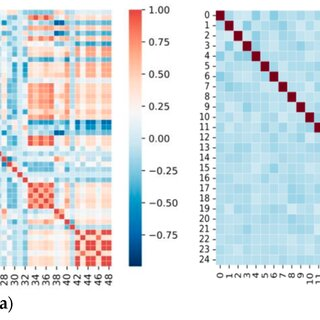
\includegraphics[width=0.4\textwidth]{assets/figures/dataset_heatmap.jpg} 
\caption{Heatmap of feature correlations in the CIC-IDS2017 dataset}
\label{fig:dataset_heatmap} 
\end{figure} 
\parencite{articlers453}

Table \ref{tab:dataset_dropna} show the information about the missing values in CIC-IDS2017. As already confirmed by the dataset shape, there are no missing values at all. In a real-world context, the impact of even small degrees of missing values may vary based on their position, patterns, and other characteristics. The absence of them can, therefore, be taken as a confirmation of the results, as CICFlowMeter, the data processing and pre-extraction tool used to create CIC-IDS2017, was designed to ensure this.


\begin{table}[H] 
\centering 
\caption{Missing Values in the CIC-IDS2017 Dataset} 
\label{tab:dataset_dropna} 
\begin{tabular}{lr} 
\toprule 
Type of Action & Number of Samples Affected \\ 
\midrule 
No Action (0 missing) & $1.25\times10^7$ \\ 
Dropna Action (776 rows) & 0 \\ 
\bottomrule 
\end{tabular} 
\end{table} 


\subsection{Preliminary EDA: Initial Impressions and Red Flags} 
The process of performing a preliminary Exploratory Data Analysis (EDA) on the CIC-IDS2017 dataset began with a high-level overview of the data structure and its constituent features. This initial step involved an immediate import of the dataset into the Python environment using the Pandas library, followed by leveraging the .info() method to succinctly display key metadata. At this juncture, the total number of records in the dataset was confirmed to be 583 days, with 78 columns, as outlined in Section \ref{subsec:ds-summary-statistics}.

Next, the focus shifted towards a more detailed examination of the dataset's features. This included a closer inspection of the data types of each column, the identification of any missing values (NaNs), and the assessment of the dataset's size in memory. The command .info(verbose=True, null\textunderscore counts=True) was instrumental in this phase, providing a verbose output that listed all the features along with their respective data types and explicit counts of missing values where applicable. The outcomes of this detailed feature analysis are systematically cataloged in Table \ref{tab:info}. For instance, it was noted that the features 'HTTPTransferSize' and 'Label' contain missing values, with counts of 6589 and 2030 missing entries, respectively.

Following the identification of missing values, the subsequent steps involved a more granular statistical analysis and a thorough examination of feature distributions. The specific commands and the resulting insights from these analyses are detailed in Sections \ref{subsec:ds-summary-statistics} and \ref{subsec:feature-dist}.


\subsection{Dataset Summary Statistics}\label{subsec:ds-summary-statistics} 
Following the preliminary EDA, a more detailed statistical analysis of the dataset was undertaken to gain deeper insights into the distributions, central tendencies, and spread of the feature values. This involved the use of the .describe() function in Pandas, which provides summary statistics for each numerical feature in the dataset. The results from this command are shown in Table \ref{tab:dataset-summary-stats}.

Table \ref{tab: dataset-summary-stats} presents an array of key statistical measures for each feature, including the count of non-null values, mean, standard deviation (std), minimum and maximum values (min and max), and quartile values (25\%, 50\%, and 75\%). These statistics are crucial for understanding the central tendencies and variability within the dataset, and they serve as a foundation for subsequent data cleaning and transformation steps. For instance, from this table, it is evident that the 'HTTPTransferSize' feature, which represents the size of data transferred during HTTP transactions, has a wide range of values with a minimum of 1 and a maximum of 40631999, and it has missing values as indicated by the count being less than the total number of records.


\subsection{Dataset Characteristics and Features} 
The CIC-IDS2017 is provided in two general file formats - raw PCAP (Packet Capture) files and processed CSV (Comma Separated Values) files containing all pre-extracted network flow features. While the former can be used in raw form, the latter pre-extracted CSV files are the generally preferred format for machine learning purposes \parencite {sharafaldin2018toward}. These CSV files were generated by using the custom-made CICFlowMeter utility, which automatically processes PCAP data to extract and calculate more than 80 different features from each observed network flow. The network flow is a single, directional communication session between a given source and destination, often uniquely identified by a five-tuple (src ip, dest ip, src port, dest port, protocol).

The individual rows in the CSV file can thus be seen as individual network flows uniquely characterised by an associated timestamp and a number of both numerical and categorical features. The full feature set provided in the processed CSV files by default is quite large, initially containing up to 84 columns (features). However, after manual inspection and following the lead of existing literature, only around 78 columns are retained, and obvious noisy columns (near-zero variance, identical values in almost all cases) are removed \parencite {kumar2021cicids}. Informatively, these features can be categorised as: 
\begin{itemize}[noitemsep] 
\item Basic Features : Flow basic information, such as Protocol (TCP/UDP/ICMP/etc. ), Flow Duration , Total Fwd Packets , and Total Backward Packets .
\item Flow Features: Statistics about the overall flow, such as Flow Bytes/s , Flow Packets/s , Flow IAT Mean (mean inter-arrival time of all packets within this flow), and Flow IAT Std (standard deviation of inter-arrival times).
\item Statistical Features of Packet Lengths: Packet size statistics such as Min Packet Length , Max Packet Length , Packet Length Mean , and Packet Length Std . These are used to detect anomalies in the fragmentation patterns or unusual payload sizes.
\item Time-Based Features (Inter-Arrival Time - IAT): Packet timing features based on inter-arrival times (IAT), such as Fwd IAT Mean and Bwd IAT Std to detect periodicity or irregularity in packet transmission.
\item Flag Counts: Counts of certain TCP flags, such as Fwd PSH Flags , Bwd PSH Flags , Fwd URG Flags , and Bwd URG Flags . These can indicate various types of control information or be used by certain types of attacks.
\item Header Lengths: Total header lengths of packets, such as Fwd Header Length and Bwd Header Length .
\item Target Label: A final column, Label , which is the explicit ground truth class. It can either be 'BENIGN', i.e. normal benign network traffic or one of the specific attack types mentioned earlier (e.g. 'DoS Hulk', 'PortScan', 'DDoS', 'Web Attack-XSS'). 
\end{itemize} 
The provision of these manually handcrafted flow-based features is quite convenient, as it saves time and effort on the initial data preprocessing steps. This would otherwise be necessary to generate all the features from raw PCAP files at the flow level before proceeding with the training \parencite {shafi2022comprehensive}. However, their inherent quality, representativeness, and potential inter-dependencies still need to be investigated, preferably in a systematic and comprehensive exploratory data analysis.

\subsection{Initial Data Exploration (EDA)} 
A systematic and comprehensive EDA was carefully conducted to better understand the dataset at hand, to diagnose and address any underlying quality issues, and to gain a deeper overall intuition for the data at hand. This iterative process of investigation included several sub-steps - the initial data load and merge, careful examination of the general structure, a more specific quality check for missingness and extreme values, and an overall statistical analysis of the feature distributions and target label.

\subsubsection{Loading and Merging Data} 
As previously noted, CIC-IDS2017 is not provided as a single file. It is thoughtfully distributed across multiple CSV files, each corresponding to a single day of network capture. The first critical step in our data analysis process was, therefore, the efficient loading of each individual CSV files into separate Pandas DataFrames. These were then merged to form a single, complete DataFrame. This crucial merging step ensured that the whole dataset was loaded and accessible as a single entity, which would then facilitate consistent and holistic analysis for all time periods combined. A few quick checks immediately after merging confirmed the presence of a total of 2,830,743 records (network flows) and 85 columns (including all the available features and the essential 'Label' column indicating the type of traffic) \parencite{al2022cicids}.

\subsubsection{Data Types and Initial Statistics} 
The second EDA step immediately after data loading, therefore, consisted of a thorough inspection of the data types of all columns. As can be expected from the output of CICFlowMeter, a vast majority of features were numerical (both integer and float). Some columns, such as the Timestamp , may load as objects (strings) and will require explicit conversion to datetime objects for any meaningful temporal analysis. However, for the primary task of flow-based classification, this can often be less critical and a lower priority. After confirming the basic structure, another crucial component of this initial EDA step involved the generation of descriptive statistics for all numerical features. This was achieved using the Pandas DataFrame.describe() function, which provided a very high-level and immediate overview of several important statistical aspects:
\begin{itemize}[noitemsep] 
\item Count : Number of non-null values for the feature. This may immediately alert for some features to any missing data issues.
\item Mean, Median (50th percentile) : Central tendency of the feature distribution. Provides a general sense of average or typical values.
\item Standard Deviation (Std): Measure of the spread or dispersion of the data around the mean.
\item Min, Max : Full range of the feature. Can be particularly useful for very quickly identifying obvious outliers, potential data entry errors, or even inherent data scaling issues.
\item Quartiles (25\textsuperscript{th}, 75\textsuperscript{th} percentiles) : Percentiles provide additional granularity to data spread. Can help understand skewness, existence of extremely high or low values outside of the central mass of the data.
\end{itemize} 
This simple yet rapid statistical summary was used to very quickly identify features with excessively large numerical ranges, some features with very low variance (unlikely to be of discriminative value), or even columns with suspicious min or max values. All these properties immediately hinted at the presence of underlying data quality issues which needed further investigation in the following steps of EDA \parencite{kumar2021cicids}.

\subsubsection{NaN (Missing Values) Treatment} 
A non-trivial and common characteristic of the dataset unequivocally discovered during the initial inspection was the presence of NaN (Not a Number) values in many features. The NaN values are often present in CIC-IDS2017 dataset because of the inability of the CICFlowMeter to compute a value for certain flow-based features due to the presence of zero-division or other issues \parencite{al2022cicids}. This can occur when there is insufficient data for the calculation, such as flows with very few packets where metrics like mean or standard deviation cannot be computed reliably. This can happen when a packet does not have certain header fields that a particular feature requires. Features like Flow Bytes/s , Flow Packets/s , and some IAT (Inter-Arrival Time) statistics were observed to contain many such NaN entries. Locating them, or rather all NaN s in the data and calculating the percentage of NaN s in each column was vital in order to assess the extent and severity of data missingness. Columns with a very high proportion of missing values (i.e. greater than 90\% or more of the records) were put aside as they were considered for outright removal. This is because any imputation on such data which is missing to a large extent will lead to either substantial bias, noise, or artificial data that would mislead a model into learning incorrect representations or patterns \parencite{mahfouz2022systematic}. This decision was to be made carefully, with an effort to keep information loss to a minimum.

\subsubsection{Inf (Infinite Values) Treatment} 
In addition to NaN s, there is a clear and equally common pattern of another peculiar characteristic of the CIC-IDS2017 dataset, which is the presence of Infinity values. These were especially common in the rate-based features, especially in Flow Bytes/s and Flow Packets/s . Such Infinity values naturally arise when the denominator in the rate calculation is approaching or equal to zero (very short flow duration), resulting in the numerical division to produce an infinite result \parencite{sharafaldin2018toward}. These Infinity values then cannot be directly processed by any machine learning algorithms and need to be addressed in a similar manner to the NaN values. The identification of all these Infinity values and the following appropriate treatment of them, therefore, was a mandatory step during the initial EDA. A common and pragmatic approach was to first replace them with NaN s (missing values) and then apply a single, consistent imputation strategy for all the forms of missing data in the next step. An alternative, careful consideration could also be given to replacing them with a very high but finite number instead, although it is more important to understand their impact on the overall distribution and to avoid introducing artificial upper bounds.

\subsubsection{Encoding Categorical Features} 
While most of the features in CIC-IDS2017 are numerical, there are two crucial columns which are in categorical form. For example, the Protocol column explicitly shows the underlying network protocol (TCP, UDP, ICMP, etc. ), which are distinct, non-ordinal categories. However, more importantly, the Label column, which is our target variable of interest, contains categorical class strings, which explicitly state whether the traffic is 'BENIGN' or is an actual attack of a specific type (e.g. 'DoS Hulk', 'PortScan', 'DDoS', 'Web Attack-XSS'). Before using any ML algorithm, these two categorical features first need to be numerically encoded or otherwise transformed to a format which can be used as input.

For the Protocol column, One-Hot Encoding (creation of new binary (0/1) columns for each unique value in the 'Protocol' feature) is the preferred and more appropriate method \parencite{al2020survey}. This is preferred over simply integer mapping of each of the unique protocols to some number because that would erroneously create an artificial ordinal relationship (e.g. that TCP is 'greater' than UDP) which would be falsely learned and leveraged by algorithms. On the other hand, for the Label column, the target for our multi-class classification, Label Encoding (mapping each unique string label to a unique integer, e.g. 'BENIGN' $\rightarrow$ 0, 'DoS Hulk' $\rightarrow$ 1, 'PortScan' $\rightarrow$ 2, etc.) is perfectly fine. This transforms the labels into a form which can directly be used by a model as the target without any unintended order.

\subsubsection{Analysis of Class Distribution} 
Possibly the most surprising and unambiguously the most important insight was gained during the initial EDA. It related to the discovery of highly unbalanced class distribution of the critical Label column. The detailed count of all unique values in this target column quite shockingly revealed that the 'BENIGN' class almost overwhelmingly (e.g. by more than 80\%) dominates the entire dataset \parencite{mahfouz2022systematic}. In other words, all samples in the dataset were around 80\% 'BENIGN' and only about 20\% are various attacks. Furthermore, while some of these attacks types may be quite common (e.g. 'Heartbleed', 'PortScan', 'DDoS'), several rare or stealthy attacks, such as 'Heartbleed', 'Infiltration', 'Web Attack-Brute Force', 'Web Attack-XSS', 'Web Attack-Sql Injection', 'Bot', etc., can be a tiny minority of the entire data. Some of these critical classes can have only a few dozen or even just a few hundred samples in the entire dataset of millions of records.

This class imbalance is an extremely important observation, as it has severe and highly negative implications for any supervised learning model we would like to train later. If not handled carefully, a model trained on this data would develop a significant bias towards the majority class 'BENIGN'. It would likely result in a high overall accuracy, but extremely low recall (true positive rate) of minority classes, which in the context of NIDS, means missing the vast majority of actual intrusions. A model that can't detect actual attacks, regardless of how well it can identify normal traffic, is not very useful or effective at all \parencite{aldhubaib2024network}. This finding immediately and strongly motivated the need for robust and carefully designed and implemented imbalance handling to be a mandatory and non-optional step during the pre-processing.

\subsubsection{Feature-Wise Analysis and Outlier Detection} 
In addition to these high-level characteristics of the overall dataset, a detailed examination of individual feature distributions was a key sub-step. This was carried out using a wide variety of powerful visualisation techniques such as histograms, box plots, and density plots. This detailed feature-wise analysis yielded several important observations about the underlying nature of the data.
\begin{itemize}[noitemsep] 
\item Skewness: A large number of features were observed to be highly skewed. That is, their values are heavily concentrated at one end of the range with a long tail towards the other. This is indicative of extreme outliers, or more generally, a very non-Gaussian distribution. For example, a number of features, like Flow Duration or Total Fwd Packets , can range from a very small value, like a few seconds or even a single packet, up to many hours or millions of packets \parencite{al2022cicids}. Many ML algorithms can struggle with such skewed distributions, or it may be necessary to transform the data before training.
\item Outliers: Box plots were also used to visually identify extreme outliers in many features. Outliers in the context of network data can originate from a number of sources. They could be either truly anomalous or malicious events (i.e. the actual intrusions we would like to detect). However, they can also be rare, benign occurrences (e.g. unusually long or very high volume legitimate connections) or, more unfortunately, can be artefacts of data collection errors. The careful decision of what to do with these outliers, whether to remove them, transform (e.g. using a log transformation), or even keep them as is, can be extremely important. It directly impacts the resulting model sensitivity, the number of false positives, and its likelihood of missing true attack patterns. The challenge is to not lose genuine anomalous attacks during outlier treatment.
\item Redundant Features: During this detailed visual inspection, several features, such as Fwd PSH Flags , Bwd PSH Flags , Fwd URG Flags , and Bwd URG Flags , were identified as having near-zero variance or even mostly zero values in practically all samples. Features with such low variance provide no or very limited useful information for a learning algorithm \parencite{kumar2021cicids}. As such, they are good candidates for removal, as they would only add computation cost without any benefit for the model's predictive capabilities.
\end{itemize} 
This comprehensive and feature-wise deep dive is extremely important to better understand what kind of data is being used as the raw material for the ML models. This is crucial to be able to make more informed and better decisions in the data cleaning and transformation steps that follow.

\subsubsection{Correlation Analysis} 
To get even more insights into the inter-feature relationships present in the dataset, the full correlation matrix was calculated, usually using Pearson correlation coefficient for each pair of numerical features, and then visualised as a heatmap for a quick and intuitive graphical representation of the linear correlations between each pair of the selected features. As expected, strong positive and negative correlations between many features were detected, which is a very common behaviour for complex network flow data. As an example, one of the most evident correlations found in many cases is between the number of Total Fwd Packets and the Fwd Header Length , as obviously sending more packets results in a larger total header length. At the same time, all different inter-arrival times often form a group of highly inter-correlated features (e.g. Flow IAT Mean and Flow IAT Max ). 

In addition to this exploratory purpose, finding strong correlations (positive or negative) between pairs of independent features is useful even for tree ensembles like XGBoost, which are usually more robust to such correlations than are linear models (regression, logistic regression, SVM, etc.). Features that are highly correlated with each other are usually either redundant or correlated with the target, but not with each other. They do not usually cause problems with tree ensembles, but can still add to the computational complexity of training and inference, and thus should still be identified in order to be able to remove one of the highly correlated features in the pair and thus simplify the model without a significant loss of information \parencite{habeeb2024two}. In this case, in-depth understanding of all such inter-feature correlations present in the CIC-IDS2017 dataset also provides even more knowledge about the flow data itself and its patterns, which can be effectively used by the NIDS.

\subsubsection{Identified Challenges and their Implications for the Methodology}
Detailed and iterative initial EDA of the CIC-IDS2017 dataset clearly revealed several critical and deeply interrelated challenges. As it was mentioned before and emphatically became apparent throughout the EDA process, these challenges are a major problem: they define and dictate all further critical and non-trivial choices that should be made in the methodology of this study, which, in the end, develops a functional NIDS based on the CIC-IDS2017 dataset.

\paragraph{1. Severe Class Imbalance} 
An enormous (extreme) imbalance in the number of benign and attack flows was one of the most important aspects of the CIC-IDS2017 dataset, as it was repeatedly shown, discussed, and especially emphasised during the EDA process. This huge difference in the number of examples in the two major classes of the dataset is by far the most significant challenge that this study is faced with and has to solve. If not properly accounted for or handled, this severe class imbalance will make it *extremely likely* for the trained machine learning model to be *highly biased* towards the *greatly overrepresented benign traffic* class. Such an imbalance will most likely result in a built NIDS that would have an *alarmingly high false negative rate (missed intrusions)* for the attack classes, which makes the NIDS unreliable in real security applications, even if its overall accuracy is high \parencite{mahfouz2022systematic}. Therefore, using at least some of the advanced imbalance handling methods that were discussed in the Section \ref{sec: bg_imbalance} becomes a requirement and a top priority when building the necessary pre-processing pipeline.

\paragraph{2. Missing and Infinite Values} 
The common (very frequent) presence of NaN and Infinity values, especially in the important rate-based features like Flow Bytes/s and Flow Packets/s , is a very significant data quality problem. The reasons for these suspicious values present in the CIC-IDS2017 dataset are the specific conditions and operations on flow records in certain corner cases (that result in 0 duration or other issues) in CICFlowMeter \parencite{sharafaldin2018toward}. Improper or inconsistent treatment of these NaN and Infinity values in pre-processing can lead to errors when training the model or even when performing data analysis, can result in noisy feature distributions, and, in general, add a significant amount of noise to the data that can confuse the learning algorithm and seriously impact its learning and final performance. Therefore, a consistent and well-justified approach to these values is clearly needed to be used in this study, including their imputation (mean, median or other imputation methods) or, in extreme cases, removal of such features from the data.

\paragraph{3. Redundant and Highly Correlated Features} 
In addition to a comparatively large number of ~78 features in CIC-IDS2017, the EDA process clearly showed a significant amount of redundancy and high inter-feature correlations between many of these features. For example, there were numerous pairs of features that contain highly similar information and are thus *multicollinear*. This is an issue that needs to be taken care of as it, among other issues, needlessly increases the computational complexity and training time of the ML model and *can also lead to decreased performance* of the ML model by either adding noise or by giving too much weight to some aspects of the input flow data \parencite{kumar2021cicids}. This also makes the interpretation of feature importance scores difficult as correlated features tend to affect each other's perceived importance scores. Therefore, either an explicit feature selection process (selecting the most discriminative features to keep and removing all others) is required or an effective intrinsic method of dealing with correlated features within the model should be used, such as XGBoost's built-in ensemble method of creating decision trees that automatically alleviates the issue to a certain extent \parencite{guha2017tutorial}.

\paragraph{4. Presence of Outliers} 
Presence of extreme outliers in the data for a number of numerical features was confirmed during the feature-wise EDA. However, the nature of these extreme outliers is still unclear: they can either be true positive or true anomalies (i.e. real intrusions, which need to be detected by the NIDS) or can be simply true benign flows, which are very rare but still possible, or finally could even be an artefact of data collection or preparation that needs to be removed from the data. All these options are reasonable and very hard to tell apart, as there is currently no direct way to look at the data and know which of the flows are indeed outliers and which ones are not. The choice of how to treat these outliers (remove them, use some transformations like a logarithm to make them less extreme or leave them alone) thus becomes a crucial and difficult question as each option will have a direct impact on the trained model's behaviour and, most importantly, on the number of false positives that it will generate. Therefore, a well-thought and clearly justified treatment of these suspicious outliers is necessary to avoid removing the true positive outliers but still handle these extreme data points in a way that they do not negatively impact the learning algorithm \parencite{al2022cicids}.

\paragraph{5. Categorical Feature Encoding} 
Finally, there were one or more categorical features, like Protocol , which need a particular way of being encoded so that the learning algorithm can easily use them and can also be sure that they do not contain any artificial relationships, such as an implicit ordering of categories for a nominal categorical feature. For example, if a simple integer mapping would be used to encode the categorical Protocol feature, the learning algorithm would probably learn and apply an ordering between these protocols, which is not present in reality and will lead to a significant drop in performance. Therefore, an appropriate encoding for nominal categorical features (like One-Hot Encoding) and separate encoding for the target Label column (like Label Encoding) will be required.

\subsubsection{Addressing EDA Insights in the Methodology} 
Insights from the very detailed and time-consuming initial dataset exploration have most definitely and to a great extent defined the rest of the study's methodology. In other words, the entire study, the methodology, which builds the proposed XGBoost-based NIDS using CIC-IDS2017, directly addresses and solves all the challenges of this dataset that were revealed during EDA.

\begin{itemize}[noitemsep] 
\item Imbalance Handling Methods: Since a class imbalance is a very serious and severe issue for this dataset, as repeatedly shown and concluded during EDA, the methodology clearly and most importantly includes techniques that effectively address it. This means a very specific and careful use of oversampling for attack classes on the training dataset (SMOTE or ADASYN for minority classes, but strictly in a way that does not cause data leakage) or, alternatively, very precise and controlled use of cost-sensitive learning through specific settings and the XGBoost algorithm itself (adjusting scale\textunderscore pos\textunderscore weight specifically for attack classes). These approaches and the required data pre-processing are, by no means, an afterthought but are, rather, absolutely critical for balanced and successful detection of all attack classes, especially the minority ones \parencite{mahfouz2022systematic}.
\item Treatment of Missing and Infinite Values: In order to remove a problem of NaN and Infinity values in the data, especially in the important rate-based features like Flow Bytes/s and Flow Packets/s , which are a common data quality issue, a very precise and robust approach to these values has to be used in this study. The first necessary step is to convert all Infinity values to NaN to have a consistent format for all missing data, and then a mean imputation method can be used to fill all NaN s with the corresponding feature's mean value. This approach was chosen because it is computationally fast and efficient and also will not alter the distribution of the values for the affected features. The effect of this imputation on the variance of features and potential bias would also be closely monitored.
\item Categorical Encoding: The use of an appropriate and precise categorical encoding for all nominal categorical features (One-Hot Encoding) and specifically separate encoding for the target Label column using Label Encoding ensures that the learning algorithm both can easily interpret the input data and is also not biased by some artificial ordinal or categorical relationships.
\item Feature Scaling: Even though tree-based models like XGBoost are robust to feature scaling, all numerical features will be standardised using StandardScaler to have a mean of 0 and standard deviation of 1. This is done to help the model with convergence when training, to make regularization more effective, and to prevent the features with larger numerical ranges from having an undue impact on the learning process.
\item Balanced Evaluation Metrics: The per-class evaluation metrics are heavily emphasised and carefully used because of the severe class imbalance in CIC-IDS2017 dataset. Due to this data issue, using simple metrics, such as overall accuracy, is clearly not enough and can be very misleading. Therefore, this study will focus more on a comprehensive set of per-class metrics , specifically detailed Precision, Recall and F1-score for *each individual attack type* as well as the 'Benign' class, and even FPR and a granular, informative Confusion Matrix . This will provide a much more reliable and actionable result of the NIDS's performance on all classes of network traffic \parencite{al2022cicids}.
\item Tuning-Informed Hyperparameter Selection: The choice of hyperparameters to tune for the XGBoost model in this study is significantly influenced by the findings from the EDA. Special attention will be given to hyperparameters that directly impact regularization (such as gamma , reg\textunderscore alpha , reg\textunderscore lambda ) and, most importantly, class weighting (such as scale\textunderscore pos\textunderscore weight ). Tuning these parameters carefully is critical to address overfitting and enhance the model's generalisation, and also to specifically handle the severe class imbalance.
\item Baseline for Comparative Analysis: A very comprehensive and detailed understanding of CIC-IDS2017 dataset, that was achieved in this very EDA section, provides a robust baseline for a later comparison of the optimised XGBoost model against other carefully selected machine learning algorithms. This will guarantee that all comparative models are trained and then evaluated on exactly the same, well-understood and appropriately pre-processed data, and thus ensure a fair and robust comparison \parencite{shafi2022comprehensive}.
\end{itemize} 
The initial extensive exploration of the CIC-IDS2017 dataset is, by no means, just a formality in this study but is, instead, an essential and crucial starting point that guarantees that all further steps in the pipeline of this machine learning study are not only technically sound and scientifically rigorous but also strategically and intimately connected to the intrinsic and complex challenges and characteristics of the selected dataset. This carefully built groundwork in turn greatly improves the overall validity, reliability, and real-world applicability of this work's results.

\subsubsection{Conclusion of Dataset Exploration} 
The initial detailed exploration of the CIC-IDS2017 dataset has most certainly and beyond reasonable doubt proven itself an immensely valuable and even an essential first step of the entire machine learning pipeline for this work. This process of data inspection and careful analysis has not only provided a wealth of critical information about the realistic composition of this dataset, including its inherent attack diversity, but also has revealed several profound and persistent challenges, including a severe class imbalance, very frequent missing and infinite values, and even a significant amount of inter-feature correlations. These important findings have then been leveraged not only to provide an actionable and deep understanding of the data's fundamental properties but also have directly informed and, most importantly, strongly justified all further decisions throughout this study's methodology, from an exact choice of necessary data pre-processing techniques all the way to a specific set of evaluation metrics. This careful and extensive preliminary analysis, in turn, forms a robust and very essential foundation that truly guarantees that the entire development and then very rigorous evaluation of the proposed XGBoost-based NIDS is firmly grounded in a very nuanced and comprehensive understanding of the dataset's unique challenges and its actual intricacies.


% ENSEMBLE LEARNING


\subsection{Deep Dive into Ensemble Learning} 

\subsubsection{Introduction} 
As we explore in this deep dive into ensemble learning, no single machine learning algorithm can be crowned as the definitive best for every possible task and dataset. Each model has its inherent advantages and weaknesses, and the choice of the "best" solution often depends on the specific context of the problem. This unpredictability and variability in model performance has led to the development and widespread adoption of ensemble learning \parencite{al2020survey}. Ensemble methods take a unique approach by combining the predictions from multiple "weak learners" to create a more powerful and accurate "strong learner." The intuition behind this approach is simple: a decision that reflects the consensus of a group of experts is usually more robust and precise than that of any individual expert, however skilled. This is especially true in complex, multi-dimensional domains like Network Intrusion Detection Systems (NIDS), where malicious patterns can be subtle and sophisticated \parencite{aldhubaib2024network}.

The ensemble strategy is backed by a strong theoretical foundation in statistics and computation. At a high level, all ensemble methods aim to reduce bias , variance , and overfitting , common issues that individual models often face. They achieve this by combining diverse models to "average out" errors, diminish the effect of noisy data, and improve the model's ability to generalize to new, unseen data. This is based on the principle that if models make different types of errors, an ensemble can reduce the overall error rate. In this chapter, we will delve into the world of ensemble learning, discussing its underlying principles, the main types of ensemble methods (bagging, boosting, and stacking), and the workings of key algorithms in each category. We will also focus on their practical application and effectiveness in the challenging domain of NIDS, drawing on recent research to highlight their importance in improving cybersecurity measures.

\subsubsection{The Basics: Foundations of Ensemble Learning} 
The primary principle driving ensemble learning is the concept of diversity . For an ensemble to outperform its individual learners, these learners must make different (or diverse ) predictions. If all base models make the same errors, combining them will not yield a better result. This diversity can be introduced in various ways:
\begin{itemize}[noitemsep] 
\item Data Manipulation: Training base models on different subsets of the training data (e.g. bootstrapping in bagging). 
\item Feature Manipulation: Training base models on different subsets of features (e.g. random feature selection in Random Forests). 
\item Algorithm Diversity: Using different types of learning algorithms as base models.
\item Parameter Diversity: Using the same algorithm but with different hyperparameters.
\end{itemize} 
The aggregation strategy then dictates how these diverse base model predictions are combined. This could be simple voting (for classification), averaging (for regression), or more complex meta-learning approaches. The power of an ensemble lies in leveraging these diverse perspectives.

\subsubsection{Bias-Variance Trade-off} 
One of the key concepts that explains the power of ensemble methods is the bias-variance trade-off . In the context of supervised learning, the total error of a model can be decomposed into three main components: bias, variance, and irreducible error. 
\begin{itemize}[noitemsep] 
\item Bias refers to the error introduced by approximating a real-world problem, which may be complicated, by a simplified model. High-bias models (e.g. linear regression on non-linear data) tend to "underfit" the training data.
\item Variance refers to the model's sensitivity to small fluctuations in the training data. High-variance models (e.g. deep decision trees) tend to "overfit" the training data, making them perform well on seen data but poorly on unseen data.
\end{itemize} 
Ensemble methods are cleverly designed to address both these issues. Methods like bagging primarily reduce variance by averaging the predictions of multiple high-variance, low-bias models. On the other hand, boosting primarily reduces bias by building models sequentially, with each new model focusing on correcting the bias (errors) of the previous models, often using low-variance, high-bias weak learners. This interplay allows ensembles to achieve a better balance in the bias-variance trade-off, leading to overall better performance \parencite{zou2021survey}.

\subsubsection{Bagging (Bootstrap Aggregating)} 
Bagging , or Bootstrap Aggregating, is one of the earliest and simplest ensemble methods, introduced by Leo Breiman in 1996. It is primarily used to reduce the variance of a prediction by generating additional data for training from the original dataset via combinations with replacement (bootstrapping). The base idea is to train several base models independently, and then combine their predictions, usually by voting for classification or averaging for regression.

\subsubsection{Bootstrapping} 
Bootstrapping is a resampling technique where subsets of the original dataset are created by drawing samples \textit{with replacement}. If the original dataset has $N$ samples, a bootstrap sample will also have $N$ samples but some of the original samples will appear multiple times, and some will not be chosen at all. This process is repeated $M$ times to get $M$ different bootstrap samples, each of which is used to train a separate base learner \parencite{agrawal2021survey}. Since each base learner is trained on a slightly different subset of the data, they will likely learn different patterns and make different errors, which is what provides the necessary diversity to the ensemble.

\subsubsection{Workings of Bagging} 
Bagging can be summarized in a few simple steps:
\begin{enumerate}[noitemsep] 
\item Draw $M$ bootstrap samples from the original training dataset.
\item Train $M$ independent base learners (typically of the same type, e.g. Decision Trees) on each of the $M$ bootstrap samples.
\item For a new, unseen data point, each of the $M$ base learners makes a prediction.
\item Aggregate the predictions: for classification, this is usually a majority vote; for regression, it's the average of the predictions.
\end{enumerate} 
By averaging (or voting) over the predictions of these diverse base learners, bagging significantly reduces the overall variance of the model, without increasing bias. It works best with complex, high-variance base models like deep Decision Trees.

\subsubsection{Random Forest (RF)} 
Random Forest (RF) is one of the most well-known and widely used bagging algorithms. It was developed by Leo Breiman in 2001 and is, in essence, an enhancement of the basic bagging approach. RF introduces an additional source of randomness into the bagging process, specifically in the tree-building process. This further decorrelates the individual Decision Trees within the ensemble and makes the RF even more resistant to overfitting than standard bagging.

\paragraph{A Closer Look} 
In Random Forest, each tree is built not only from a bootstrap sample of the data but also by considering only a random subset of features at each split point within the tree \parencite{almutairi2025intrusion}.
\begin{enumerate}[noitemsep] 
\item For each of the $M$ trees: 
\begin{itemize}[noitemsep] 
\item A bootstrap sample of the training data is drawn.
\item At each node of the tree, instead of considering all available features for the best split, only a random subset of $k$ features is considered. The optimal choice of $k$ is typically $\sqrt{p}$ for classification (where $p$ is the total number of features) and $p/3$ for regression.
\item The Decision Tree is grown to its maximum depth without pruning (or with very minimal pruning), as the ensemble's averaging effect will take care of any overfitting.
\end{itemize} 
\item For prediction, the output is simply aggregated: majority vote for classification, average for regression. 
\end{enumerate} 
This two-level randomness (data sampling and feature sampling) ensures that the individual trees are diverse and do not overfit to specific features, which results in an extremely powerful and generalizable model.

\paragraph{RF in the NIDS: Strengths} 
Random Forest's advantages make it particularly well-suited for NIDS:
\begin{itemize}[noitemsep] 
\item Reduction in Overfitting: The ensemble nature and two-level randomness of RF provide excellent immunity against overfitting, which is crucial when dealing with noisy and high-dimensional network traffic data \parencite{almutairi2025intrusion}.
\item High Predictive Accuracy: RF consistently achieves high predictive accuracy across a wide range of NIDS tasks, from binary (attack/benign) to multi-class classification of different attack types \parencite{shafi2022comprehensive}.
\item Feature Importance Insights: RF inherently provides a measure of feature importance (e.g. Gini importance or permutation importance), which helps to identify the most discriminative network flow features for intrusion detection, which is a valuable insight for security analysts \parencite{wang2023efficient}.
\item Handles High-Dimensionality Well: RF can perform well even when the number of features is large, as it only considers a subset of them at each split.
\item Robustness to Noise and Outliers: The aggregation of many trees makes it less sensitive to individual noisy data points or outliers than single models would be.
\end{itemize} 

\paragraph{Limitations} 
RF, despite its many strengths, has its own set of limitations:
\begin{itemize}[noitemsep] 
\item Less Interpretable: While individual Decision Trees are highly interpretable, an ensemble of hundreds or thousands of trees becomes a "black box", making it difficult to explain the reasoning behind specific intrusion alerts.
\item Computational Cost: Training many trees can be computationally expensive and time-consuming, particularly for very large datasets and deep trees.
\item Bias towards Categorical Features: Can be biased towards features with more categories when computing feature importance.
\end{itemize} 

\paragraph{Applications and Impact in NIDS} 
RF has been used extensively in NIDS research and has shown impressive results. For example, in \parencite{shafi2022comprehensive}, RF's robust performance across various NIDS datasets is highlighted. In \parencite{wang2023efficient}, RF's efficacy in classifying network intrusions is demonstrated, often outperforming traditional machine learning algorithms due to its ability to handle complex feature interactions and data noise. More recent studies on the CIC-IDS2017 dataset have continued to find RF as a strong contender for accurate intrusion detection, especially when dealing with multi-class classification problems with diverse attack types \parencite{almutairi2025intrusion}. It has also been used for feature selection by leveraging its built-in feature importance, which can help build more lightweight and efficient NIDS models.

\subsubsection{Boosting} 
Boosting is the opposite of bagging's parallel, independent training of multiple models. In boosting, models are built sequentially, with each new model focusing on correcting the errors made by the previous ones. The main idea is to iteratively train "weak learners" (models that are only slightly better than random guessing) and combine them into a strong learner. The key is that each new weak learner is trained to give more attention to the data points that the previous models misclassified or handled poorly, thus sequentially improving the overall model's performance. The primary goal of boosting is to reduce bias and transform many weak, simple models into a single, highly accurate one \parencite{friedman2001greedy}.

\subsubsection{The General Principle of Gradient Boosting Machines (GBM)}
Most modern boosting algorithms are built on the core concept of Gradient Boosting Machines (GBM) \parencite{chen2016xgboost}. The fundamental idea behind GBM is to combine weak learners (most commonly, Decision Trees, specifically "regression trees") by fitting each new tree to the residuals (errors) of the previous step. Rather than fitting the new tree directly to the original target variable, the new tree is fit to the negative gradient of the loss function with respect to the current model's predictions. This iterative process allows the model to progressively reduce the loss function, building an ensemble that specifically targets the remaining errors. GBM has several key characteristics: 
\begin{itemize}[noitemsep] 
\item Sequential Learning: Trees are added one at a time, and the previous trees remain unchanged.
\item Loss Function Optimization: The process is driven by minimizing a differentiable loss function (e.g. mean squared error for regression, logarithmic loss for classification).
\item Weak Learners: Simple models, usually shallow Decision Trees (stumps or trees with few splits), are used as base learners.
\item Shrinkage (Learning Rate): Each new tree's contribution to the ensemble is scaled by a small learning rate, which helps prevent overfitting and improve generalization.
\end{itemize} 
From this general framework, several highly optimized and popular boosting algorithms have been developed, revolutionizing machine learning.

\subsubsection{Extreme Gradient Boosting (XGBoost)} 
XGBoost (eXtreme Gradient Boosting) is a highly optimized, scalable, and powerful implementation of the gradient boosting framework. Created by Tianqi Chen, it has gained massive popularity and often achieves state-of-the-art performance in a wide range of machine learning competitions and real-world applications since its release \parencite{chen2016xgboost}. XGBoost builds on the core ideas of GBM and introduces several important enhancements that significantly improve its efficiency, scalability, and predictive power.

\paragraph{Inside the Black Box} 
XGBoost's remarkable performance is due to a combination of algorithmic and system-level optimizations:
\begin{enumerate}[noitemsep] 
\item Regularization: Unlike traditional GBM, XGBoost includes explicit L1 (Lasso) and L2 (Ridge) regularization terms in its objective function. These regularization terms penalize the complexity of the model (e.g. the number of leaves and the magnitude of leaf weights), which actively prevents overfitting and encourages model generalization. This is a key feature, especially for noisy data like network traffic \parencite{habeeb2024two}.
\item Advanced Tree Construction: XGBoost uses a 'level-wise' or 'depth-wise' tree growth strategy, also known as Exact Greedy Algorithm or Approximate Greedy Algorithm for large datasets. It also uses a smart split-finding algorithm that includes sparsity-aware split finding, which can efficiently deal with missing values and zeroes by learning the best direction for missing values.
\item Shrinkage and Column Subsampling: Like GBM, XGBoost also uses a learning\textunderscore rate (or eta ) to shrink the contribution of each individual tree, preventing any one tree from dominating the overall prediction and making the learning more conservative. It also uses column subsampling (like Random Forest's feature bagging) to randomly select a subset of features for each tree, which further reduces variance and speeds up computation \parencite{almutairi2025intrusion}.
\item Tree Pruning: XGBoost uses a 'max\textunderscore depth' parameter and a gamma parameter. gamma specifies the minimum loss reduction required to make a further partition on a leaf node. If a split does not meet this threshold, it is pruned. This allows for much more effective pruning than the traditional greedy algorithm, which only prunes after the tree is fully grown.
\item Handling Missing Values: XGBoost can automatically learn the best way to handle missing values by having default directions for splits when a value is missing, which is highly useful for real-world datasets where missingness is a common occurrence.
\item Parallel Computing: At a system level, XGBoost is designed to support parallel processing of tree construction. While trees are added sequentially, the inner loops (e.g. finding the best split for a node) can be parallelized across CPU cores, which can greatly speed up training.
\end{enumerate} 

\paragraph{Key Advantages} 
\begin{itemize}[noitemsep] 
\item High Accuracy: Consistently provides state-of-the-art predictive performance across a wide range of classification and regression tasks.
\item Robustness against Overfitting: The built-in regularization, shrinkage, and column subsampling mechanisms offer strong protection against overfitting.
\item Scalability and Efficiency: Designed for parallel computation and efficient memory usage, making it highly effective for large datasets.
\item Handles Missing Data Automatically: Its sparsity-aware split finding can intelligently handle missing values without requiring explicit imputation beforehand (although pre-imputation can still be helpful).
\item Flexibility: Supports custom objective functions and evaluation metrics, allowing it to be tailored to specific problem needs.
\item Feature Importance: Provides robust feature importance scores, which can help in understanding the factors that drive predictions.
\end{itemize} 
\subsubsection{Computational Complexity and Resource Requirements} 
Ensemble methods, especially those involving large numbers of deep trees like Random Forests or boosting algorithms like XGBoost, are computationally intensive. They require significant CPU and memory resources for both training and inference \parencite{aldhubaib2024network}. This can be particularly challenging in real-time or near-real-time NIDS, where decisions need to be made swiftly as packets arrive. Deploying these models in operational environments may necessitate high-performance computing infrastructure or optimisations that can scale with the massive, streaming nature of network data.

\subsubsection{Model Complexity and Interpretability} 
The increased complexity that comes with ensembles can lead to models that are difficult to interpret. Understanding the basis for an ensemble's decision can be more challenging than with simpler models. In the context of NIDS, where explaining or auditing decisions may be necessary for network forensics or compliance reasons, this lack of interpretability can be a significant drawback. Techniques to improve interpretability, like feature importance rankings or model-agnostic interpretation methods, may need to be applied, but these can add overhead and may not fully resolve the issue \parencite{liu2021improving}.

\subsubsection{Integration with Existing Infrastructure} 
Deploying ensemble-based NIDS into existing network security architectures can be non-trivial. It may require changes to data handling processes, updates to integration with other security tools (like SIEM systems), or adaptations in network hardware to support the required computational load. Careful consideration must be given to how these systems interface with current infrastructure, including considerations around data privacy and security, especially when deploying to environments with stringent regulatory requirements \parencite{albanese2021integrating}.

\subsubsection{Overfitting with Improper Tuning} 
While ensemble methods are less prone to overfitting, they are not immune, particularly if improperly configured. Using too many models in an ensemble, especially deep or complex ones, can lead to overfitting to the noise in the training data rather than underlying attack patterns. In NIDS, where the availability of labelled attack data can be limited, there's a risk of building a system that performs well on known threats but poorly on novel or emerging ones. Regularisation, careful tuning of ensemble size, and validation against diverse and representative datasets are essential to mitigate this \parencite{gautam2021overfitting}.

\subsubsection{Maintaining Performance with Evolving Threats} 
The effectiveness of an NIDS can degrade over time as attackers adapt and develop new techniques. While ensemble methods are generally good at generalisation, continuously evolving the ensemble model to keep pace with new types of network traffic and attack strategies can be challenging. This might involve regular retraining, updating the model with new data, or dynamically adjusting ensemble composition. Such maintenance requires ongoing effort and expertise to ensure the NIDS remains effective \parencite{khan2021ensemble}.

\subsubsection{Dataset Specificity and Transferability} 
Ensemble models can sometimes be very specific to the datasets on which they were trained. Transferring a model from one network environment to another, or from one type of network traffic to another, can lead to a drop in performance if the underlying data distributions differ significantly. This issue of transferability is particularly acute in NIDS, where the operational environment and traffic patterns can vary widely from the conditions seen in training datasets \parencite{wang2023transferability}.

\subsubsection{Hyperparameter Tuning and Configuration} 
Ensemble learning algorithms come with a range of hyperparameters that need to be tuned for optimal performance. This tuning process can be complex and computationally expensive, particularly for large ensembles or those using sophisticated base learners. In NIDS, where the cost of false negatives (missed intrusions) can be high, finding the right configuration that balances sensitivity, specificity, and computational efficiency is crucial but non-trivial \parencite{li2022challenges}.

\subsubsection{Increased Computational Cost and Training Time} 
The most direct drawback of ensemble methods is that they generally have a higher computational cost and require longer training times compared to using single models. Bagging and Random Forest involve training several independent models, while boosting trains models sequentially. Stacking, with its multi-layered architecture and cross-validation for meta-feature generation, is typically the most computationally expensive \parencite{aldhubaib2024network}. This can be a significant challenge, especially with very large NIDS datasets or in environments where models must be deployed or retrained frequently.

\subsubsection{Reduced Interpretability (Black-Box Nature)} 
While Decision Trees are known for their interpretability, the ensemble of many trees (Random Forest, XGBoost, LightGBM, CatBoost) or the combination of different model types (stacking) leads to a more "black-box" approach. It becomes significantly harder to interpret exactly *why* a decision was made or *which specific features* were responsible for a given intrusion alert \parencite{kasongo2021improving}. This reduced transparency can affect trust and adoption among security analysts, hamper troubleshooting and post-incident analysis, and also complicate efforts to reverse-engineer attack techniques, pointing to an important research direction of Explainable AI (XAI) for NIDS.

\subsubsection{Hyperparameter Complexity} 
Ensemble methods, particularly gradient boosting algorithms like XGBoost, LightGBM, and CatBoost, involve numerous hyperparameters that can greatly affect performance. Finding the right balance for these parameters (learning rate, tree depth, regularization terms, subsampling rate, etc.) is critical but can be a complex and time-consuming process, often involving exhaustive grid search, random search, or more sophisticated Bayesian optimization. Suboptimal hyperparameter settings can lead to underfitting or, more problematically, overfitting, thus degrading the performance of the NIDS \parencite{habeeb2024two}.

\subsubsection{Vulnerability to Adversarial Attacks} 
Like other machine learning models, ensemble methods, including deep learning ensembles, can be vulnerable to adversarial attacks. Adversaries can craft subtle, often imperceptible perturbations to network traffic (adversarial examples) that lead the ensemble NIDS to misclassify malicious traffic as benign (evasion attacks) or as a different type of attack. The added complexity of ensemble models can sometimes make them more difficult to defend against certain adversarial manipulations, as vulnerabilities might be distributed across the different base learners \parencite{kim2021adversarial}.

\subsection{Conclusion} 
Ensemble learning is a major shift in the way we approach machine learning problems. Instead of relying on the strengths of a single model, we can combine multiple models to compensate for individual weaknesses, leading to more accurate, stable, and generalizable machine learning systems. Bagging methods like Random Forest work by averaging out the predictions of independently trained models on bootstrapped datasets, thus reducing variance. Boosting algorithms, such as the highly optimized XGBoost, LightGBM, and CatBoost, build models sequentially to focus on and correct the errors of previous learners, effectively reducing bias and achieving high performance. Advanced methods like stacking can further improve performance by using a meta-learner to optimally combine the predictions of diverse base models.

Ensemble learning offers several significant benefits in the context of Network Intrusion Detection Systems. It helps improve the accuracy of detection by harnessing the combined power of multiple models, it enhances robustness by reducing the likelihood of being evaded by complex attack patterns, and it addresses class imbalance by effectively leveraging information from both minority and majority classes. Feature importance analysis offered by ensembles provides valuable insights into the nature of network traffic and intrusions. Ensembles also help in improving the generalization ability of NIDS to unseen and novel threats. However, challenges such as increased computational requirements, reduced interpretability, hyperparameter tuning complexity, and vulnerability to adversarial attacks remain. Nevertheless, ongoing research and development of techniques like Explainable AI (XAI) and real-time hyperparameter optimization are actively addressing these issues and will continue to refine and reinforce the role of ensemble learning in building advanced, resilient, and adaptive NIDS for our increasingly interconnected world.



% DEEP DIVE INTO XGBOOST
\subsection{Deep Dive into XGBoost: Principles, Advantages, and Hyperparameters}

\subsubsection{Introduction to XGBoost} 
In today's fast-evolving machine learning landscape, where the quest for highly accurate, scalable, and efficient predictive models is unending, one algorithm stands out as a stalwart: XGBoost, which stands for eXtreme Gradient Boosting. Since its introduction by Tianqi Chen in 2016 \parencite{chen2016xgboost}, it has not only been a winner in numerous data science competitions but also found its way into production in a wide variety of real-world applications, ranging from fraud detection and recommendation systems to, most relevant to this dissertation, Network Intrusion Detection Systems (NIDS) \parencite{almutairi2025intrusion, habeeb2024two}. The reasons for its widespread popularity are not arbitrary; they are the fruits of a sophisticated algorithm design that carefully balances predictive performance, computational efficiency, and scalability.

XGBoost is an implementation of the broader family of Gradient Boosting Machines (GBM) \parencite{al2020survey}. However, what truly distinguishes it and earns it the moniker "eXtreme" are the numerous algorithmic and system-level optimizations that dramatically improve its performance, robustness, and speed. These improvements help it scale to large datasets, handle missing values, and reduce the dreaded overfitting, all the while maintaining state-of-the-art accuracy. For the challenging, high-stakes problem of NIDS, where enormous volumes of noisy, high-dimensional, and often highly imbalanced network traffic data must be sifted through to detect rare and sophisticated cyber threats, XGBoost provides a compelling, highly effective solution \parencite{aldhubaib2024network}. This chapter is an in-depth study of XGBoost, where its core principles are explained, unique advantages are highlighted, and most importantly, the effects of key hyperparameters are described in detail.

\subsubsection{Core Principles of XGBoost} 
In order to understand XGBoost, one must first be familiar with a few key concepts: ensemble learning, gradient boosting, and the choice of the base learner (weak learner). These concepts form the backbone of this powerful learning algorithm.

\subsubsection{Ensemble Learning and Boosting} 
XGBoost is based on the principle of ensemble learning, a machine learning paradigm that combines the predictive power of multiple "weak learners" to create a more accurate and robust "strong learner" \parencite{zou2021survey}. This "wisdom of the crowd" often leads to superior predictive performance than any of the individual models could achieve on their own. XGBoost is a part of a specific class of ensemble methods known as boosting algorithms.

Unlike bagging methods (like Random Forest, for example), which train several models independently of one another and then average their outputs to create the ensemble, boosting algorithms build their ensemble in a sequential, additive manner. Each new weak learner in a boosting ensemble is trained to improve upon the performance of the existing ensemble of learners. This sequential refinement of the ensemble allows the model to focus more and more on the "difficult" data points that the current ensemble finds hard to predict, iteratively reducing the ensemble's overall error \parencite{agrawal2021survey}. The end goal of boosting is to reduce bias: take many weak, simple (and hence low-variance and high-bias) models and transform them into one single, more complex and powerful model.

\subsubsection{Gradient Boosting Machines (GBM)} 
The immediate precursor to XGBoost is a machine learning algorithm known as the Gradient Boosting Machine (GBM). The idea behind it is to frame the problem of ensemble learning as an optimisation problem of minimising some differentiable loss function \parencite{chen2016xgboost}. In other words, instead of training a new weak learner on the residuals (or the difference between the actual target value and the prediction from the previous iteration of the model), GBM fits each new tree to the negative gradient of the loss function with respect to the current ensemble's predictions.

Suppose the current ensemble model at step $m$ is $F_m(x)$ and the next new weak learner to be added to it is $h_m(x)$, then the updated model is given by $F_{m+1}(x) = F_m(x) + \gamma_m h_m(x)$, where $\gamma_m$ is a step size. The new weak learner $h_m(x)$ is then trained to predict the "pseudo-residuals," which is proportional to the negative gradient of the loss function $L(y, F_m(x))$ with respect to $F_m(x)$:
$$ r_i = -\left[\frac{\partial L(y_i, F_m(x_i))}{\partial F_m(x_i)}\right]_{F_m(x)} $$ 
This ensures that the new tree is explicitly pushing the ensemble model towards a more optimal solution, and this process is repeated many times, thus minimising the overall loss function. The continuous refinement of the model is directly aimed at the parts where the model is performing poorly, resulting in large reductions in the prediction error.

\subsubsection{Decision Trees as Weak Learners} 
In XGBoost and most GBM implementations, the weak learners are almost exclusively Decision Trees, and more specifically, "regression trees". These are typically shallow trees, often called 'stumps' or trees of some small, pre-specified maximum depth. The choice of decision trees as the weak learner is deliberate for several reasons:
\begin{itemize}[noitemsep] 
\item Non-linearity: Trees can model complex non-linear relationships and interactions between features, which is essential for modelling complex datasets like network traffic.
\item Interpretability (Individual Tree): While the entire ensemble can be a black-box model, individual shallow trees are relatively easy to interpret.
\item Robustness: They are robust to feature scaling and can handle mixed types of data (numerical and categorical features).
\item Efficiency : Training shallow trees is computationally efficient. 
\end{itemize} 
Each new tree is optimised to learn the errors in the predictions of the previous ensemble and its contribution is often "shrunk" by a learning rate to ensure a conservative, gradual improvement and to also prevent overfitting \parencite{zou2021survey}.

\subsubsection{XGBoost: Algorithmic Enhancements and Mechanics} 
It is the algorithmic and system-level improvements to the basic GBM architecture that make XGBoost special. XGBoost is the result of many such improvements that were carefully designed and optimised to provide top-notch performance, speed, and scalability.

\subsubsection{Regularization in the Objective Function} 
One unique feature of XGBoost that sets it apart from most GBM implementations is the inclusion of explicit regularization terms in the objective function itself. While most previous GBM algorithms would resort to tree pruning for regularisation, XGBoost's objective function for the $t^{th}$ iteration is given by:
$$ \mathcal{L}^{(t)} = \sum_{i=1}^{n} l(y_i, \hat{y}_i^{(t-1)} + f_t(x_i)) + \Omega(f_t) $$ 
Where $l$ is the differentiable loss function (usually squared error loss or cross-entropy loss), $f_t(x_i)$ is the new tree being added, and $\Omega(f_t)$ is the regularisation term for the new tree. This regularisation term typically consists of L1 and L2 penalties:
$$ \Omega(f_t) = \gamma T + \frac{1}{2} \lambda \sum_{j=1}^{T} w_j^2 $$ 
Where $T$ is the number of leaves in the tree, $w_j$ is the weight (prediction) of leaf $j$, $\gamma$ is the L1 regularisation term, and $\lambda$ is the L2 regularisation term.
\begin{itemize}[noitemsep] 
\item L1 Regularization ($\alpha$ or reg\textunderscore alpha ): The L1 penalty term biases the optimisation algorithm to prefer trees with fewer leaves and feature interactions (simple trees with fewer splits), and can also be useful in feature selection as it pushes the weights of some feature paths towards zero.
\item L2 Regularization ($\lambda$ or reg\textunderscore lambda ): The L2 term discourages large leaf weights, and in a way smooths out the model by reducing its reliance on individual instances, helping the model to generalise better and thus combat overfitting \parencite{habeeb2024two}.
\end{itemize} 
By building these explicit penalties for model complexity into the objective function itself, XGBoost naturally builds simpler, more generalisable trees, which is an extremely powerful way of guarding against overfitting, especially for noisy, high-dimensional datasets such as network traffic.

\subsubsection{Sparsity-Aware Split Finding} 
Datasets, especially in areas such as NIDS, are often likely to contain sparse features or a large number of missing values \parencite{kumar2021cicids}. XGBoost is specifically designed to deal with these efficiently via a sparsity-aware split-finding algorithm. Instead of requiring explicit imputation of missing values prior to training (though this may still be required for some types of features before training), XGBoost learns the best direction for missing values at each split. For every feature and for each potential split, the algorithm learns two default directions for missing values: one that sends all missing values in the left child, and the other that sends them to the right child. The optimal default direction (minimising the loss) is then selected, thus learning to handle missing values for each feature \parencite{chen2016xgboost}. This not only simplifies the data preprocessing pipeline, but can often lead to more robust models as well as the algorithm has explicitly accounted for the value (or lack thereof) of missing features.

\subsubsection{Approximate Greedy Algorithm and Weighted Quantile Sketch} 
For large datasets that do not fit in memory, computing the exact best split at every single node of every tree can be infeasible. XGBoost instead uses an Approximate Greedy Algorithm \parencite{chen2016xgboost}. Instead of searching all the possible split points to find the exact best split, this algorithm proposes a set of candidate split points. It does so by building a "weighted quantile sketch" over the distribution of the feature, and then searching for the best split among these candidate split points only. This drastically reduces the computation time while still yielding very high accuracy. The weights in the weighted quantile sketch correspond to the second-order gradients so that the algorithm is biased towards splits that are more likely to reduce the objective function.

\subsubsection{Shrinkage (Learning Rate)} 
One extremely useful method of regularisation that is often used in gradient boosting to prevent overfitting (and is also used in XGBoost) is called shrinkage, and is controlled by the learning\textunderscore rate (or eta ) hyperparameter. The effect of this hyperparameter is to shrink the contribution of each new tree added to the ensemble by a small factor equal to the learning rate. In other words, it scales down the predictions of each new tree by the value of the learning rate. This means that each successive tree has more "room" to fit the errors left by the previous ensemble of trees, resulting in a more conservative, gradual training process \parencite{aldhubaib2024network}. A smaller learning rate often requires a greater number of trees ( n\textunderscore estimators ) to train but usually results in a better, more robust model with better generalisation performance. It also acts as a regularisation mechanism, as no single tree is allowed to dominate the ensemble or over-correct the errors.

\subsubsection{Column Subsampling (Feature Bagging)} 
As in Random Forest, XGBoost also employs column subsampling (also known as feature bagging). At each boosting round (that is, at each new tree being built), only a random subset of the available features are considered for the best split. This has two effects: 
\begin{itemize}[noitemsep] 
\item Reduces Overfitting: By introducing a random element in the choice of features, it helps prevent individual trees from over-fitting to specific features and thus improves the robustness of the ensemble.
\item Speeds up Computation: Evaluating fewer features at each split greatly speeds up the tree-building process.
\end{itemize} 
XGBoost has various options for column subsampling: colsample\textunderscore bytree (subsample features per tree), colsample\textunderscore bylevel (subsample features per split level), and colsample\textunderscore bynode (subsample features per node), allowing fine-grained control over this regularisation mechanism \parencite{almutairi2025intrusion}.

\subsubsection{Tree Pruning} 
XGBoost has a unique tree pruning strategy. Rather than greedily grow each tree to some maximum depth and then prune it back (post-pruning), XGBoost has the ability to do pre-pruning using the gamma parameter. gamma specifies the minimum loss reduction required to make a further partition on a leaf node. If a potential split does not provide a sufficient loss reduction as specified by gamma , it will simply not be made. This direct approach to pruning usually results in faster tree construction and also prevents overfitting by not allowing unnecessary complex branches \parencite{chen2016xgboost}.

\subsubsection{Parallel Computing} 
Although the boosting process itself is sequential in nature (trees are built one after the other), XGBoost can still achieve significant speedups through parallel computation at the system level. The inner loop of tree construction (finding the best split for each node) is the most time-consuming part, and XGBoost parallelizes this step so that different features or different data instances can be processed in parallel across multiple CPU cores. This system-level parallelization is a primary reason it can handle very large datasets so efficiently, which makes it practical for high-volume NIDS \parencite{agrawal2021survey}.

\subsubsection{Advantages of XGBoost} 
The combination of the algorithmic and system-level enhancements gives XGBoost several unique advantages that make it very powerful for computationally demanding and large-scale problems such as network intrusion detection.

\subsubsection{Superior Accuracy} 
XGBoost has state-of-the-art predictive accuracy for a wide variety of classification and regression tasks. Its gradient boosting framework coupled with strong regularization means it can learn highly complex data patterns and interactions which lead to very precise predictions. In a NIDS context, that high accuracy is paramount since even a small improvement in the detection rate can translate to a major improvement in the overall cybersecurity posture of an organization \parencite{aldhubaib2024network}.

\subsubsection{High Speed and Scalability} 
The "eXtreme" in XGBoost is, in many ways, a result of its impressive speed and scalability. Thanks to its parallelization capabilities, optimized tree-learning algorithms (approximate greedy algorithm, weighted quantile sketch, etc), and efficient memory usage, XGBoost can train on large datasets of sizes that would overwhelm most other algorithms \parencite{chen2016xgboost}. This efficiency is of course critical for a NIDS that is expected to handle enormous volumes of network traffic in real-time or near real-time settings.

\subsubsection{Robustness Against Overfitting} 
XGBoost is quite resistant to overfitting, a common problem for complex models that tend to memorize training data. This is in large part because of its multi-pronged regularization strategy with:
\begin{itemize}[noitemsep] 
\item Explicit L1 and L2 regularization in objective function
\item Shrinkage (learning rate) to make the learning process more conservative
\item Column subsampling to inject some randomness 
\item Tree pruning to cut off the growth of a tree when the improvement in loss is not significant
\end{itemize} 
All this means the final model generalises well to unseen data. This is of course a key necessity for intrusion detection since it is necessary to detect novel or otherwise unknown cyber threats that were not explicitly present in the training set \parencite{habeeb2024two}.

\subsubsection{Effective Handling of Missing Values} 
Unlike many other algorithms that require manual pre-imputation of missing values or even better that are robust to missing values, XGBoost has an inherent ability to handle them with its split-finding algorithm that is sparsity-aware. It learns the direction of missing values for each split in training and hence often comes with models that are better robust without any additional preprocessing overhead \parencite{al2020survey}. This is no small advantage for real-world network traffic datasets which are likely to contain missing or undefined features.

\subsubsection{Flexibility and Customization} 
XGBoost is quite flexible, allowing for custom objective functions and evaluation metrics. Researchers and engineers can, in fact, tailor the model closely to the specific requirements of the problem at hand. In the NIDS setting, this would mean one could optimize for particular metrics such as recall (to minimize false negatives or missed attacks) or even a balanced F1-score rather than just overall accuracy, which is especially useful when dealing with imbalanced classes (attacks v/s normal) \parencite{shafi2022comprehensive}.

\subsubsection{Built-in Feature Importance} 
Built into XGBoost is a reliable way to obtain the importance of each feature in making predictions. The feature importance scores can be quite invaluable for gaining insight into the underlying patterns behind intrusions, like what are the most important network flow attributes that help in distinguishing malicious activity from normal traffic. This can inform security teams about the most relevant aspects to monitor and even act as a form of actionable intelligence for network administrators and security analysts \parencite{almutairi2025intrusion}.

\subsubsection{Cross-Platform Compatibility} 
XGBoost is available in many different programming languages (Python, R, Java, Scala, C++). This makes it accessible to a larger community of developers and researchers and also helps with its integration into a variety of existing security systems and frameworks.

\subsubsection{Key Hyperparameters and Their Impact} 
Effectively tuning XGBoost to achieve high performance for a specific task, like a NIDS, depends greatly on understanding the various hyperparameters that the model exposes to the user and tweaking them to match the characteristics of the dataset at hand. XGBoost's hyperparameters control almost all aspects of the learning process, from the depth of the trees and regularization amounts to the learning rate and data subsampling. Choosing the right set of hyperparameters is very important; setting them inappropriately can lead to a model that underfits or overfits or is just very inefficient during training.

In a nutshell, XGBoost hyperparameters fall into 3 main categories: General Parameters, Booster Parameters, and Learning Task Parameters.

\subsubsection{General Parameters} 
These parameters govern the general working of XGBoost.

\begin{itemize}[noitemsep] 
\item booster : Specifies the booster to be used. Can be gbtree (tree-based), gblinear (linear model), or dart (Dropouts meet Multiple Additive Regression Trees). The default value for this hyperparameter is gbtree , which is almost always the recommended setting due to its much higher accuracy and the non-linear relationships that tree-based models are able to capture. Note that the regularisation parameters apply only to gbtree , so setting this to something else would likely lead to overfitting.

\item nthread (or n\textunderscore jobs in the scikit-learn wrapper): Number of parallel threads to be used when running XGBoost. Setting it to equal the number of CPU cores available will typically result in a major speedup in training. The default value for this hyperparameter is to use as many CPU cores as are available.

\end{itemize} 

\subsubsection{Booster Parameters (Tree-Specific Parameters for gbtree )} 
These parameters control the tree-specific hyperparameters and are used to regularize and tune the decision trees themselves. These are the hyperparameters that are most commonly tuned in a typical XGBoost usage.

\begin{itemize}[noitemsep] 
\item eta (or learning\textunderscore rate ) : 

\begin{itemize}[noitemsep] 
\item Description : Step size shrinkage used to prevent overfitting. At each boosting step, this is used to scale the contribution of the current tree before it is added to the previous trees. In other words, after a new tree is fit, its feature weights are multiplied directly by eta .
\item Impact: This smaller eta values lead to a more conservative boosting process which needs more boosting iterations n\textunderscore estimators but often leads to more robust models. Higher eta values allow the model to learn faster, but the risk of overfitting is higher.
\item Tuning Strategy: This is almost always set to a small value such as 0.01, 0.05, 0.1, 0.2, 0.3, etc, and is tuned in conjunction with n\textunderscore estimators .
\end{itemize} 

\item max\textunderscore depth : 

\begin{itemize}[noitemsep] 
\item Description : Maximum depth of a tree. It controls the complexity of the model by constraining the amount of room each tree has to grow.
\item Impact: More depth allows each tree to capture more complex feature interactions and non-linearities but, unsurprisingly, at the cost of a much higher risk of overfitting. Shallower trees lead to simpler models that are far more robust.
\item Tuning Strategy: This is one of the most important hyperparameters to tune in order to control overfitting. It is very commonly tuned within a range of [3, 10] for most problems. With network intrusion data in particular, it is almost always a good idea to start with moderate tree depths and then, if necessary, increase cautiously from there.
\end{itemize} 

\item gamma (or min\textunderscore split\textunderscore loss ) : 

\begin{itemize}[noitemsep] 
\item Description: Minimum loss reduction required to make a further partition on a leaf node of the tree. You can think of it as similar to the concept of information gain used in decision trees.
\item Impact: Larger values make the algorithm more conservative by pruning splits that do not lead to a sufficient decrease in loss. It is used as a kind of threshold for pruning.
\item Tuning Strategy: This is commonly tuned in ranges such as [0, 0.1, 0.2, 0.5, 1.0]. It can be an effective regularization hyperparameter to tune alongside max\textunderscore depth .
\end{itemize} 

\item subsample : 

\begin{itemize}[noitemsep] 
\item Description: Fraction of training instances (rows) to be randomly sampled for each tree.
\item Impact : Setting this to less than 1.0 (e.g. 0.7, 0.8) introduces randomness into the model, decreasing its variance, which in turn prevents overfitting (this is the exact same idea as the bagging ensemble method).
\item Tuning Strategy: This is most commonly tuned within a range of [0.5, 1.0]. Lower values decrease the variance of the model, but introduce more bias.
\end{itemize} 

\item colsample\textunderscore bytree , colsample\textunderscore bylevel , colsample\textunderscore bynode : 

\begin{itemize}[noitemsep] 
\item Description: These parameters control the subsampling of columns (features). Specifically, 
\begin{itemize} 
\item colsample\textunderscore bytree: Fraction of columns to be randomly sampled for each tree.
\item colsample\textunderscore bylevel: Fraction of columns to be randomly sampled for each level (depth) in a tree.
\item colsample\textunderscore bynode: Fraction of columns to be randomly sampled for each split node.
\end{itemize} 
\item Impact : Same concept as subsample . Introduces randomness in the selection of the features. By making the individual trees more diverse, this reduces variance and thus helps prevent overfitting.
\item Tuning Strategy: Usually tuned in a range of [0.5, 1.0]. They can often be tuned together for a more powerful regularization effect.
\end{itemize} 

\item lambda (or reg\textunderscore lambda ) : 

\begin{itemize}[noitemsep] 
\item Description : L2 regularization term on weights. Note that this is not to be confused with lambda\textunderscore vartype below.
\item Impact: Penalizes large leaf weights by adding their L2 squared value to the objective. This makes the model more conservative (less sensitive to the individual training instances) and helps reduce overfitting.
\item Tuning Strategy: This is typically tuned within a wide range (powers of 10 are good) such as [1, 10, 100, 1000].
\end{itemize} 

\item alpha (or reg\textunderscore alpha ) : 

\begin{itemize}[noitemsep] 
\item Description : L1 regularization term on weights. Note that this is not to be confused with alpha\textunderscore vartype below.
\item Impact: Encourages sparsity in the leaf weights (often leads to simpler models), acting as a form of feature selection from within the tree-structure. This also helps prevent overfitting. 
\item Tuning Strategy: This hyperparameter is often tuned within a range such as [0, 0.001, 0.01, 0.1].
\end{itemize} 

\item num\textunderscore parallel\textunderscore tree : 

\begin{itemize}[noitemsep] 
\item Description: This is only used for Random Forest mode in XGBoost. If you set it to a value > 1, XGBoost will grow multiple trees in parallel for each boosting iteration.
\item Impact: This essentially turns the XGBoost boosting algorithm into some kind of Random Forest-like ensemble.
\item Tuning Strategy : Set this to 1 for typical boosting. 
\end{itemize} 

\end{itemize} 
\subsubsection{Learning Task Parameters} 
These parameters set the optimization objective and evaluation metrics.
\begin{itemize}[noitemsep] 
\item objective : 
\begin{itemize}[noitemsep] 
\item Description : Specifies the loss function to be minimised. 
\item Common Values for NIDS : 
\begin{itemize} 
\item binary:logistic : Binary classification with probability output. 
\item multi: softmax : Multi-class classification with predicted class label output. Requires num\textunderscore class parameter. 
\item multi: softprob : Multi-class classification with predicted class probabilities for each class output. Requires num\textunderscore class parameter. 
\end{itemize} 
\item Impact: Directly dictates the optimization target for the model. Correctly setting the objective for your NIDS task (binary vs. multi-class) is critical.
\end{itemize} 

\item eval\textunderscore metric : 
\begin{itemize}[noitemsep] 
\item Description : Metric for evaluating the model during validation. 
\item Common Values for NIDS (especially with imbalance) :
\begin{itemize} 
\item logloss : Negative log-likelihood. 
\item error : Binary classification error rate (1 - accuracy). 
\item merror : Multi-class classification error rate. 
\item auc: Area under the ROC curve (binary classification only).
\item auprc: Area under the Precision-Recall curve (great for imbalanced datasets).
\item Custom metrics (e.g., F1-score, Recall for minority classes).
\end{itemize} 
\item Impact: Determines early stopping criteria and provides an interpretable target for hyperparameter tuning. For imbalanced NIDS datasets, F1-score (macro or weighted) or AUPRC are more informative than plain accuracy.
\end{itemize} 

\item seed (or random\textunderscore state ) : 
\begin{itemize}[noitemsep] 
\item Description : Random seed for reproducibility. 
\item Impact: Guarantees that the results from multiple runs are identical if all other parameters are unchanged.
\end{itemize} 

\item scale\textunderscore pos\textunderscore weight : 
\begin{itemize}[noitemsep] 
\item Description: Weight balancing factor between positive and negative instances. Highly useful for severely imbalanced binary classification tasks.
\item Impact: Raises the relative weight of the minority class (positive class), compelling the model to focus more on it, thereby increasing recall for the minority class. Should be set to (sum(negative instances) / sum(positive instances)) \parencite{habeeb2024two}. For multi-class, more elaborate weighting may be required, or resorting to external resampling techniques on the training set instead.
\item Tuning Strategy: A very important parameter for NIDS as the attacks are the minority classes. Either use the formula above or tune it carefully.
\end{itemize} 
\end{itemize} 

\subsubsection{Tuning Strategy Implications for NIDS} 
The tuning of XGBoost for NIDS must be conducted with a specific strategy in mind that takes into account domain-specific considerations, most notably the severe class imbalance typically present and the critical need to maximize recall of true intrusions while controlling the false positive rate.
\begin{itemize}[noitemsep] 
\item Prioritize Metrics: Metrics like macro-averaged F1-score, weighted F1-score or Area Under the Precision-Recall Curve (AUPRC) on the validation set should be prioritized over overall accuracy during tuning. The recall for individual attack classes is often also of critical interest and should be tracked.
\item Address Imbalance Early: scale\textunderscore pos\textunderscore weight should be set early for binary classification. For multi-class problems, internal class weighting or external resampling techniques (e.g., SMOTE) applied to the training set are often necessary.
\item Regularization for Generalization: Due to the expected noisiness of network data, heavy regularization (tuning gamma , lambda , alpha , subsample , colsample\textunderscore bytree ) is often beneficial to prevent overfitting to training noise and to ensure the model generalizes well to unseen attacks.
\item Iterative Tuning : A common iterative tuning pipeline is: 
\begin{enumerate} 
\item Tune n\textunderscore estimators and learning\textunderscore rate (begin with a moderate learning\textunderscore rate and use it to find an optimal n\textunderscore estimators with early stopping).
\item Tune max\textunderscore depth and min\textunderscore child\textunderscore weight (related to gamma ).
\item Tune subsample and colsample\textunderscore bytree . 
\item Tune regularization ( lambda , alpha ). 
\item Re-tune learning\textunderscore rate and n\textunderscore estimators with the new parameters.
\end{enumerate} 
\item Cross-Validation: Hyperparameter tuning should always be done using cross-validation (e.g., 5-fold or 10-fold) on the training set in order to get a robust performance estimate and to avoid overfitting to a single validation set split.
\end{itemize} 

\subsubsection{XGBoost in Network Intrusion Detection (NIDS)} 
XGBoost's unique combination of algorithmic excellence and practical efficiency makes it exceptionally well-suited for the demanding and critical application of Network Intrusion Detection (NIDS) \parencite{aldhubaib2024network}. At the core, the key strengths of XGBoost directly map to and help overcome many of the enduring challenges found in NIDS:
\begin{itemize}[noitemsep] 
\item Handling Massive Datasets: Network traffic data is generated in massive quantities. XGBoost's scalability and efficient use of computational resources allow NIDS to process these vast datasets in a tractable manner, a must-have feature for real-world applications \parencite{almutairi2025intrusion}.
\item Diverse and Complex Attack Detection: The nature of cyberattacks is inherently diverse and complex. XGBoost's ensemble method, built upon learning non-linear patterns with multiple decision trees, is highly capable of capturing the breadth of intrusion types, from simple port scans to more complex DoS/DDoS attacks and web exploits \parencite{habeeb2024two}.
\item Class Imbalance Mitigation: Class imbalance, where benign traffic significantly outweighs attack instances, is a notorious problem in NIDS. XGBoost's scale\textunderscore pos\textunderscore weight parameter and support for external resampling methods (when needed) provide robust tools for rebalancing the learning process and ensuring that the detection of critical minority attack classes is given high recall \parencite{mahfouz2022systematic}.
\item Robustness and Generalization: The strong regularization in XGBoost leads to models that are less prone to overfit to noise in the training data. This results in a robust and generalizable NIDS, capable of detecting novel or mutated variants of known attacks, a key requirement in mitigating zero-day threats \parencite{agrawal2021survey}.
\item Actionable Insights (Feature Importance): The model's feature importance scores are not just algorithmic byproducts; they provide actionable intelligence. They help security analysts to pinpoint which network flow features contribute most significantly to detecting malicious activity, thereby offering a data-driven way to improve network monitoring, security policies, and to gain insights into the evolving landscape of attacks \parencite{kasongo2021improving}.
\end{itemize} 
Leveraging these capabilities and systematically tuning its hyperparameters for the task at hand enables researchers and practitioners to build and deploy highly effective and resilient NIDS based on XGBoost that can make a real difference to an organization's overall cybersecurity resilience.



% Existing Research on NIDS using XGBOOST 


\subsection{Identification of Research Gaps}

The thorough literature review has examined the latest developments in Network Intrusion Detection Systems (NIDS), highlighting the effectiveness of Machine Learning (ML), particularly XGBoost \parencite{aldhubaib2024network}. We've explored its core principles, benefits like speed and accuracy, and how its hyperparameters function \parencite{chen2016xgboost, habeeb2024two}. The review also assessed its successful application on challenging datasets like CIC-IDS2017, along with common pre-processing and feature engineering methods \parencite{almutairi2025intrusion, kumar2021cicids}.

However, this analysis goes beyond summarising existing knowledge; it aims to pinpoint areas that need further investigation. Finding these research gaps is crucial for creating a novel and valuable contribution \parencite{mahfouz2022systematic}. This section identifies specific areas where current research falls short, justifying the need for this dissertation and defining its potential impact on ML-based NIDS.

\subsubsection{Pinpointing Specific Research Gaps for Contribution}
Building on the existing literature, this section systematically identifies specific gaps where this research can make a unique and significant contribution. These areas present opportunities to improve the effectiveness of XGBoost-based NIDS.

\subsubsection{Novel Pre-processing Techniques, particularly Adaptive Imputation for Multi-Class}
Although standard pre-processing methods are widely used, there's a lack of research into new or adaptively combined strategies for diverse NIDS datasets like CIC-IDS2017. Current imputation methods, like using the mean or median, may not be optimal for skewed data or when missing values are meaningful. Furthermore, while techniques like `scale\textunderscore pos\textunderscore weight` and SMOTE address class imbalance, the literature lacks a comprehensive analysis of multi-class-specific imbalance handling. The challenge is not just applying SMOTE but dynamically determining optimal oversampling ratios for each minority class or developing more granular cost-sensitive strategies. This research will address this gap by investigating:
\begin{itemize}[noitemsep]
	\item \textit{Adaptive and Context-Aware Imputation}: Exploring imputation strategies that consider the context of the missing value.
	\item \textit{Optimized Multi-Class Resampling Integration}: Comparing different sophisticated oversampling and undersampling techniques for each minority class in CIC-IDS2017 and their interaction with XGBoost's capabilities.
	\item \textit{Outlier-Aware Pre-processing}: Developing pre-processing pipelines that differentiate between genuine anomalous attacks and noise to avoid removing critical attack patterns.
\end{itemize}

\subsubsection{Optimized XGBoost Hyperparameter Tuning with Multi-Class Imbalance in Mind}
Identification of Research Gaps 
The literature review chapter has already explored some of the freshest, cutting-edge developments in the domain of NIDS, briefly demonstrated the usefulness and success of ML in general, and XGBoost in particular \parencite{aldhubaib2024network}. We have investigated the inner workings of its base principles, advantages such as its speed and accuracy, and how its hyperparameters impact the way the ensemble algorithm functions \parencite{chen2016xgboost, habeeb2024two}. The literature review also encompassed a swift assessment of the successful applications on extremely challenging datasets (such as CIC-IDS2017), as well as all of the preprocessing and feature engineering methods that are most commonly used in this particular field by ML researchers \parencite{almutairi2025intrusion, kumar2021cicids}.

At this point, it is worth noting that the literature review serves not only as an aggregation and concise summary of past and present knowledge on the topic of research; but most importantly, it is meant to further enable a thorough evaluation of the state of the art in the given field by identifying the areas in need of additional study – in other words, finding the research gaps \parencite{mahfouz2022systematic}. This section of the dissertation precisely aims to point out the particular areas in which a noticeable void has been left by other researchers, thereby justifying the existence of this body of work, and allowing it to specify its potential contribution to the fields of ML and, more specifically, ML-based NIDS.

Pinpointing Specific Research Gaps for Contribution 
The present section, serving as an extension to the previous one, methodically identifies the specific gaps in the literature that the present research would aim to make a novel and non-trivial contribution to, and therefore, present open opportunities for further improvement of the effectiveness of an XGBoost-based NIDS solution.

Novel Pre-processing Techniques, particularly Adaptive Imputation for Multi-Class
Standard pre-processing methods have become quite routine among the related data science community, but the research has been surprisingly scarce regarding either new or adaptively combined pre-processing pipelines for multi-class (and inherently more diverse in terms of data features) NIDS datasets such as CIC-IDS2017. The prevailing imputation strategy based on a relatively simple mean or median substitution can be far from ideal in scenarios with skewed data or when the missing value itself is significant (as is often the case in ML-based NIDS). In addition, while a number of techniques such as `scale\textunderscore pos\textunderscore weight` and SMOTE were demonstrated to address the challenge of class imbalance, the related literature was lacking in both sophisticated, hyperparameter-free analysis of the specificities of multi-class imbalance, and an in-depth empirical exploration of how a multi-class imbalance should be addressed in terms of XGBoost-based solutions. That is, the actual challenge of applying SMOTE (as well as its alternatives) is not necessarily in its implementation, but rather in identifying the optimal upsampling/downsampling ratio for each minority class in multi-class CIC-IDS2017, or potentially developing more fine-grained cost-sensitive alternatives. This dissertation would close this gap by further exploring:
\begin{itemize}[noitemsep] 
\item \textit{Adaptive and Context-Aware Imputation}: Conducting a search for alternative imputation strategies that take into account the circumstances under which the information was lost in the first place (if applicable).
\item \textit{Optimized Multi-Class Resampling Integration}: A thorough comparative empirical investigation of various sophisticated oversampling and undersampling methods for each minority class in CIC-IDS2017, and a dedicated study of the possible ways in which these methods can affect or be affected by XGBoost's own native capabilities.
\item \textit{Outlier-Aware Pre-processing}: In the context of outlier (or invalid) handling, further development of the NIDS data pre-processing pipeline in the sense that it can distinguish between the true anomalous nature of genuinely malicious attacks vs. mere invalid or otherwise ‘rubbish' data that is better off being discarded so as not to remove critical patterns of attack.
\end{itemize} 

Optimized XGBoost Hyperparameter Tuning with Multi-Class Imbalance in Mind
The body of research that focuses on tuning XGBoost hyperparameters for NIDS invariably aims for an overall improvement of the accuracy scores, while almost none of them reported a detailed breakdown of how the hyperparameters had been tuned in the context of multi-class imbalance on CIC-IDS2017. A noticeable research gap is therefore: 
\begin{itemize}[noitemsep] 
\item \textit{Multi-Objective Tuning for Imbalance}: Developing and applying tuning strategies that jointly optimise for multiple objectives, such as maximising the recall for the smallest minority class at the same time as minimising the overall false positive rate.
\item \textit{Dynamic `scale\textunderscore pos\textunderscore weight` for Multi-Class}: A study of advanced hyperparameter tuning strategies for `scale\textunderscore pos\textunderscore weight` that would allow it to be set more dynamically for each minority class.
\item \textit{Impact of Regularization on Imbalance}: A more thorough empirical study of the effects of the XGBoost's regularization hyperparameters in the context of handling class imbalance and their interaction with class weighting techniques as a way to prevent overfitting.
\end{itemize} 

Focus on Specific Attack Types within CIC-IDS2017 
While overall detection rates can be high, XGBoost and its previous iterations are still seemingly unable to recognise specific rare attack types within CIC-IDS2017 as precisely as other attacks (examples include `Heartbleed`, `Infiltration` \parencite{kumar2021cicids, al2022cicids}, etc.). A particular research gap to be explored therefore is:
\begin{itemize}[noitemsep] 
\item \textit{Targeted Optimization for Minority Attacks}: Identifying attack-specific optimal tuning strategies, which can include attack-specific feature engineering, and/or a unique subset of the full spectrum of hyperparameters (the latter is required by `catboost`) to target the ‘weakest points' of the algorithm for each type of difficult-to-detect attacks.
\item \textit{Detailed Error Analysis}: A more granular error analysis specifically for each type of challenging attacks with a view to using the produced insights as a direct indicator of where to focus the model-improvement effort in the next iteration.
\item \textit{Attack-Specific Thresholding}: An empirical evaluation of adaptive attack-specific thresholding strategies (i.e. optimising each attack type's precision-recall trade-off individually rather than for the NIDS as a whole).
\end{itemize} 

Addressing Class Imbalance Effectively: A Deeper Contribution 
The issue of class imbalance is well-recognised \parencite{mahfouz2022systematic, aldhubaib2024network}, yet there has been a dire lack of a rigorous approach to what is meant by an `effectively addressed' imbalance, specifically in the context of multi-class XGBoost. That is, there is a further research gap that can be explored in much greater detail, and which could form the central part of this dissertation, presented as follows:
\begin{itemize}[noitemsep] 
\item \textit{Comparative Efficacy of Imbalance Techniques with XGBoost}: An empirical comparison of the state of the art imbalance handling techniques when coupled with the XGBoost classifier for multi-class CIC-IDS2017 in order to come to a reasoned conclusion regarding the most efficacious imbalance addressing strategy for each attack type. That is, empirical evidence of what is best suited for which type of data, rather than an anecdotal or heuristic approach.
\item \textit{Optimizing Balance Ratios}: An empirical search for the optimal (and potentially, different for each attack type) balance ratio.
\item \textit{Impact on Generalization and Robustness}: How different imbalance handling techniques affect the model's generalization performance and its robustness against overfitting, in both short and long terms (in the latter sense, also related to the hyperparameter tuning).
\end{itemize} 
The idea of this dissertation, and its core contribution to the field, will therefore be to provide a systematic investigation of what the most effective ways are to address the problem of multi-class class imbalance within the context of XGBoost for CIC-IDS2017, supported by robust, empirical evidence of the validity of the proposed strategies.

